\chapter{Design} \label{chapter:design}
During the design stage, we set out research questions and detail the steps of the machine learning pipeline for diagnosing fault types in the MaFaulDa dataset. The explanatory analysis of MaFaulDa hints at the underlying dependencies within feature sets that can degrade the machine learning model of choice. We apply the methodology for vibration measurements from standards to the data logger requirements and data acquisition from industrial equipment.

\section{Research questions}
The thesis aims to provide answers to five research questions. The main focus is on making data flow more efficient in an industrial sensor network that monitors rotating machines. The \textbf{research questions} are:
\begin{enumerate}[label=RQ\arabic*., font=\bfseries]
    \itemsep0pt
	\item Which time-domain and frequency-domain features are extractable from vibrations to provide the most accurate record of machinery faults?
	\item What is the reduction in transmission goodput with signal features?
	\item What accuracies of fault classification are achievable with tiny feature subsets?
	\item How do the vibration signals collected on the industrial machinery behave?
	\item How can machinery faults be identified over time from collected events?
\end{enumerate}

\noindent In accomplishing the objectives of our research, we propose several \textbf{goals}:
\begin{todolist}
    \itemsep0pt
    \item Statistically and visually describe vibration signals from the Machinery fault database (MauFaulDa).
    \item Establish a list of conditions that will be investigated later in the experimental setting.
    \item Prepare the dataset to be used in conjunction with machine learning models namely by identifying labels and balancing classes.
    \item Find the best subsets of features in the time and frequency domain with previously analyzed feature extraction and selection methods.
    \item Evaluate the performance of models described in the diagnostics section with a significant focus on the k-nearest neighbor algorithm.
    \item Acquire measurements of vibrations from machines in the real environment to form a novel dataset of machinery behavior.
    \item Develop hardware and implement its firmware to obtain such measurements of the quality demanded by vibrodiagnostics standards.
\end{todolist}

\section{Machine learning pipeline}
The similar data processing framework we adopt can be found elsewhere in the literature. It generally consists of signal acquisition, feature extraction, dimensionality reduction, and pattern recognition or fault detection~\cite{wang_bearing_2015}. However, the realization of the steps must be decomposed closer to suit the dataset structure, desired processing goals, and investigated parameters. The entire design of the data flow can be seen in Fig.~\ref{fig:design:ml-pipeline}.

\begin{figure}[h]
    \centering
	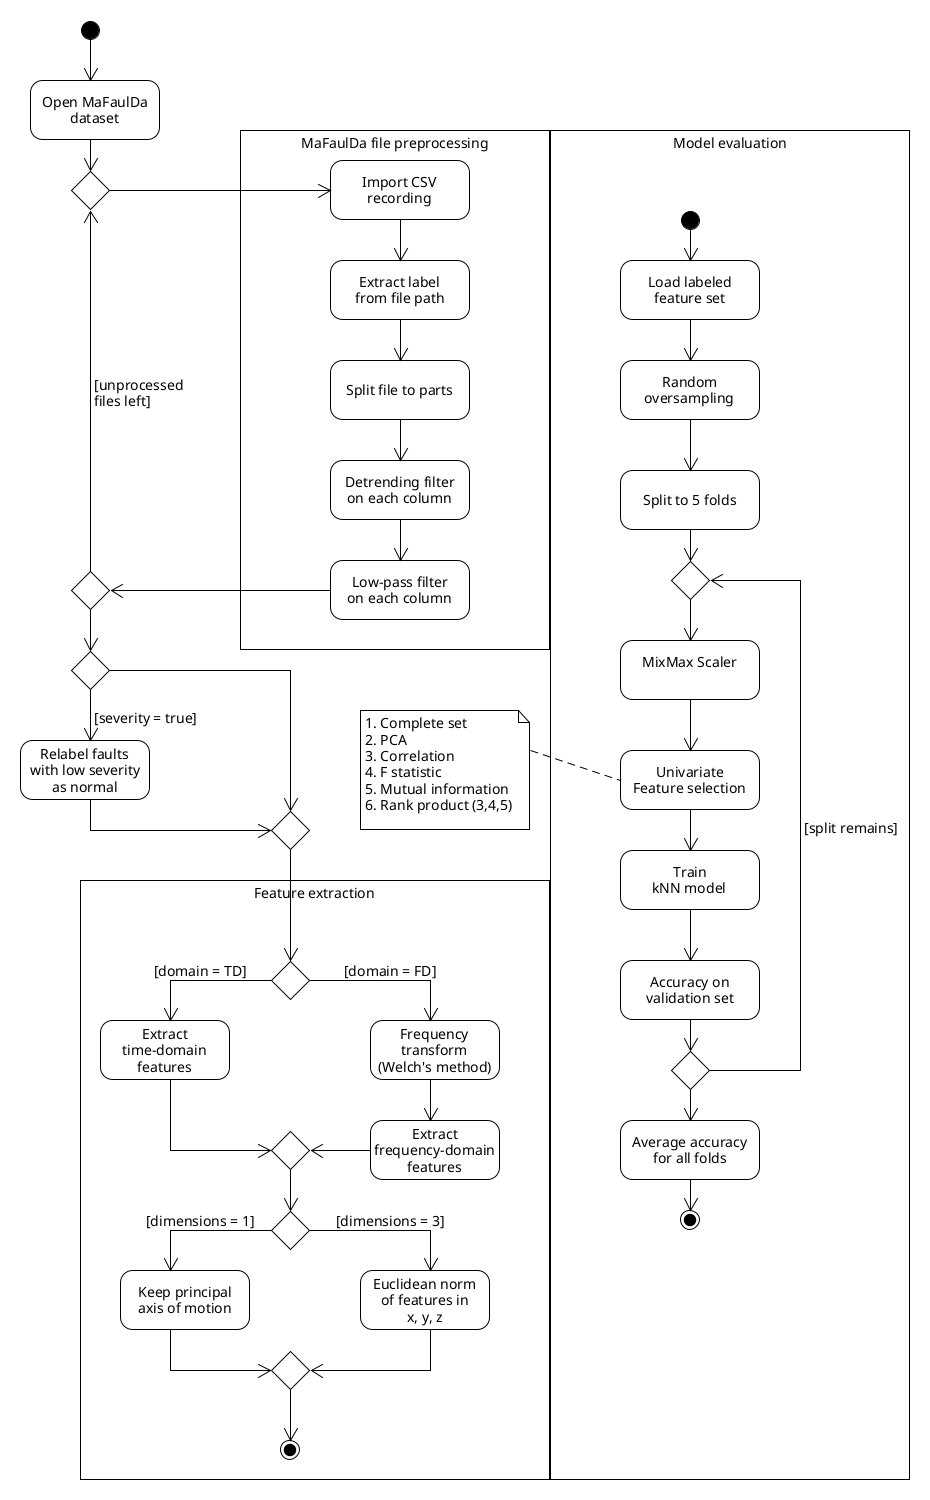
\includegraphics[width=0.9\textwidth]{assets/design/pipeline-design.png}
	\caption{Machine learning pipeline for MaFaulDa dataset}
	\label{fig:design:ml-pipeline}
\end{figure}
\afterpage{\clearpage}

\textbf{In preprocessing step}, the signals stored in columns of CSV files within the MaFaulDa ZIP archive are first associated with metadata according to the file's path in the directory structure. The hierarchically topmost folder describes the simulated defect. There is directory for \emph{normal}, \emph{imbalance}, \emph{horizontal-misalignment}, \emph{vertical-misalignment}, \emph{overhang} (outer bearing), \emph{underhang} (inner bearing). Each bearing has an additional folder layer for dividing bearing faults: \emph{ball\_fault}, \emph{cage\_fault}, \emph{outer\_race}. Each fault category except the normal class contains various fault severities with units of grams or millimeters. The severities in turn consist of individual files with different rpm speeds. 

We neglect the \textbf{acceleration sensor orientation}, therefore, the labels for shaft misalignment in vertical and horizontal directions are merged into the same group. In the end, that leaves \textbf{6 types of labels}: baseline, two shaft faults are imbalance and misalignment, and three bearing faults are cage fault, ball fault, and outer race fault.  

Depending on the \textbf{chosen bearing position}, only time series associated with that bearing are retained because the standards demand each bearing be assessed separately. Fault classification concerns bearing in direct contact and shaft mechanically passing through it.

The strength of the recorded response to the underlying defect is dependent on the shaft \textbf{rotational speed}. Speed in units of rpm is calculated from pulsed speedometer output. It is the average distance between two successive rising edges:
\begin{ceqn}\begin{align}
\mathrm{rpm} = 60 \;/\; \overline{\Delta t}
\end{align}\end{ceqn}

\textbf{File description} is the triplet of \textbf{fault}, \textbf{severity}, and \textbf{rpm}.

After labeling we insert a step to split the time series into parts when the duration is long enough to introduce more observations artificially. This assumption for splitting is not met for MaFaulDa because, for the desired frequency resolution for features of close to 1~Hz, we need a window size of 32768 samples. Variation reduction in spectral estimation brings the necessity to average at least 12 overlapping windows. The full length of 5 seconds provides 15 whole overlapping windows. 

The \textbf{DC component} in the three-dimensional vibration signal is removed by subtracting the global mean. Immediately follows a digital IIR Butterworth low pass filter of \nth{5} order with cutoff frequency 10 kHz at -3 dB. Before the usage of a low pass filter, the peak at 20 kHz with a sideband was present as an unwanted artifact. It could not have been reliably recorded due to the linear frequency response of the sensor up to 10 kHz. At the same time, such a frequency is outside the range of any feasible MEMS accelerometer.

\textbf{Initial labels can be exchanged} for a label of fault-free state when the severity is low. The count of severity levels is not identical in every group. The numerical amounts for each level are sorted in ascending order within each fault and then these levels are normalized using a min-max scaler.

The preprocessed signal from each axis of accelerometer is packed up to \textbf{two base feature sets} in time domain (TD) and frequency domain (FD). The feature extraction formulas are is identical with formulas presented in the section \ref{section:feature-extraction} of analysis chapter. The frequency transform is Welch's method averaging FFT vectors from 32768 samples after Hann windowing and 50\% overlap. The feature sets are:
\begin{itemize}
\itemsep0pt
\item \textbf{TD has 10 time-domain features} - peak-to-peak amplitude (\emph{pp}), zero-crossing rate (\emph{zerocross}), root mean square (\emph{rms}), skewness, kurtosis, shape factor, crest factor, impulse factor, clearance factor, average amplitude change (aac), 
\item \textbf{FD has 11 frequency-domain features} - spectral centroid, standard deviation (\emph{std}), skewness, kurtosis, roll-on frequency, roll-off frequency, spectral flux, noisiness, spectral negentropy, energy, entropy.
\end{itemize}
 
The four conditions are applied in the instance of the pipeline to filter observations with calculated features to create \textbf{24 scenarios}:
\begin{itemize}
\itemsep0pt
\item \textbf{Source bearings} - samples and fault labels are left in either just for the inner bearing (A), for only the outer bearing (B), or for both bearings (A+B).
\item \textbf{Feature domain} - the set of extracted features as an input to downstream models is changed either to TD or FD set,
\item \textbf{Accelerometer axis} - Either one principal direction of motion or all three dimensions is aggregated under same feature name (1 or 3),
\item \textbf{High severity faults} - to more precisely simulate fault frequencies found in real environment the low severity defects can be considered as normal operation (Yes or No).
\end{itemize}

The \textbf{fault classification} performance metrics are evaluated after balancing classes feature normalization, and 5-fold cross-validation validation on the k-nearest neighbor classifier with Euclidean distance metric. The population of classes is evened out with random oversampling using a strategy to resample all but the majority class. In the multi-class classification, the micro-averaged performance metrics of accuracy, precision, and recall result in the same number. Therefore, accuracy is only one on the output. 

The hyperparameter of k-neighbours and a feature subset size are tweaked, and results are compared under different preprocessing conditions and in multiple experiments:

\begin{itemize}
\itemsep0pt
\item \textbf{Complete feature sets}: compare the accuracy of the k-NN model in relation to the k-value as an odd number in the range from 1 to 37 on the dataset under different conditions. The TD and FD sets are treated separately.

\item \textbf{Feature combinations} - every combination of feature subsets with 2, 3, and 4 members are evaluated to obtain the statistical distribution of all possible k-NN models. The k-value is sequentially increased from options 3, 5, and 11 neighbours. The single k-value generates $\sum_{j=2}^{4}{\binom{n}{j}}$ where $n$ is number of members in complete feature set. In total 375 models for TD and 550 models for FD are tested under identical conditions. 

The observed effect is a rate of decrease in accuracy while shrinking the number of features to the bare minimum. The side product is finding the global optimum by brute force of the most informative attributes in predicting the defect.

\item \textbf{Feature selection methods} - the choice of feature subset is performed in linear time complexity as opposed to exponential in combinatorial case. The dimensionality reduction using \textbf{principal components analysis} (PCA) does further extraction and retains only the components that best explain the variance. The disadvantage is that the resulting linear combination cannot be interpreted easily. 

The best feature subset from complete sets is picked after ranking the features according to their importance. The bivariate scores for ranking are the mean of point biserial \textbf{correlation} to every class label as a dichotomous variable, \textbf{Fisher score} (F statistic), and \textbf{Mutual information}. The correlation among features can reduce model's prediction power. The rank product combines the three latter scores into the ensemble. The comparison for the accuracy of the feature selection strategy is made in relation to the entire model accuracy distribution. 

\item \textbf{Incremental learning} - the order of samples tries to simulate the gradually worsening state of the machine and delayed annotation of defects. Observations are sorted based on increasing relative severity. The faults within levels are shuffled randomly. 

The \textbf{tumbling window} of lengths 1, 10, 100 measurements imitates regular expert visits annotating observations recorded until that moment. Labels for the whole previous window are supplied at once.

Another common problem with online learning is \textbf{missing annotations} due to the size of the dataset. The equal-length gaps of 0, 2, 10, and 50 labels are skipped before another observation is annotated. This approach of skipping samples without considering their representativeness can harm the predictions. 
\end{itemize}

The experimental design involves the filter conditions that create 24 forms of the original MaFaulDa. The four main experiments test hyperparameters on each dataset variation. Those are k-neighbors, a number and kind of features in batch learning tumbling windows, and label skips in incremental learning.

\section{Exploratory data analysis of MaFaulDa}
A better explanation for model behavior is arranged by examining the number of observations per fault category, spatial separability of the distinguished groups, and scales of the attributes and their interdependencies.

Out of the 1951 time series, the inner bearing (A) has 1438, and the outer bearing (B) has 1393~(Tab.~\ref{tab:design:label-count}). Source bearing A+B just concatanes observations from both postions so the column sums their counts together. The observations for shaft defects are shared regardless of the bearing. 
\begin{table}[h]
\renewcommand{\arraystretch}{1.2}
\centering
\begin{tabular}{|ll|r|r|r|r|r|r|}
\hline
\multicolumn{2}{|l|}{\textbf{Source bearing}}                                            & \multicolumn{1}{l|}{A}  & \multicolumn{1}{l|}{A+B} & \multicolumn{1}{l|}{B}  & \multicolumn{1}{l|}{A}   & \multicolumn{1}{l|}{A+B} & \multicolumn{1}{l|}{B}   \\ \hline
\multicolumn{2}{|l|}{\textbf{High severity faults}}                                & \multicolumn{1}{l|}{No} & \multicolumn{1}{l|}{No}  & \multicolumn{1}{l|}{No} & \multicolumn{1}{l|}{Yes} & \multicolumn{1}{l|}{Yes} & \multicolumn{1}{l|}{Yes} \\ \hline
\multicolumn{1}{|l|}{\multirow{6}{*}{\textbf{Fault}}} & \textbf{misalignment}     & 498                     & 996                      & 498                     & 248                      & 496                      & 248                      \\ \cline{2-8} 
\multicolumn{1}{|l|}{}                                & \textbf{imbalance}        & 333                     & 666                      & 333                     & 188                      & 376                      & 188                      \\ \cline{2-8} 
\multicolumn{1}{|l|}{}                                & \textbf{cage fault}       & 188                     & 376                      & 188                     & 91                       & 181                      & 90                       \\ \cline{2-8} 
\multicolumn{1}{|l|}{}                                & \textbf{ball fault}       & 186                     & 323                      & 137                     & 87                       & 132                      & 45                       \\ \cline{2-8} 
\multicolumn{1}{|l|}{}                                & \textbf{outer race fault} & 184                     & 372                      & 188                     & 86                       & 176                      & 90                       \\ \cline{2-8} 
\multicolumn{1}{|l|}{}                                & \textbf{normal}           & 49                      & 98                       & 49                      & 738                      & 1470                     & 732                      \\ \hline
\multicolumn{2}{|l|}{$\Sigma$}                                                    & \textbf{1438}           & \textbf{2831}            & \textbf{1393}           & \textbf{1438}            & \textbf{2831}            & \textbf{1393}            \\ \hline
\end{tabular}
\caption{Number of observation in MaFaulDa split by class label according to source bearing}
\label{tab:design:label-count}
\end{table}

The fusion of vertical and horizontal misalignment gives rise to the label that occurs the most at 34.63\%. The baseline class is the least populous at 3.4\% for the inner bearing. After relacing low severity faults with the normal status it became the largest with 51.32\%. The imbalance ratio as a proportion of the largest to the smallest classes is 10.16 for original labels and 8.58 after relabeling.

Exemplary waveforms from each fault class illustrate their
superficial differences in oscillatory behavior. The files with the highest severity levels and around an average rotational speed of 2500 rpm (42 Hz) are displayed to discern patterns.
\begin{figure}[h]
    \centering
    \begin{subfigure}[b]{0.48\textwidth}
        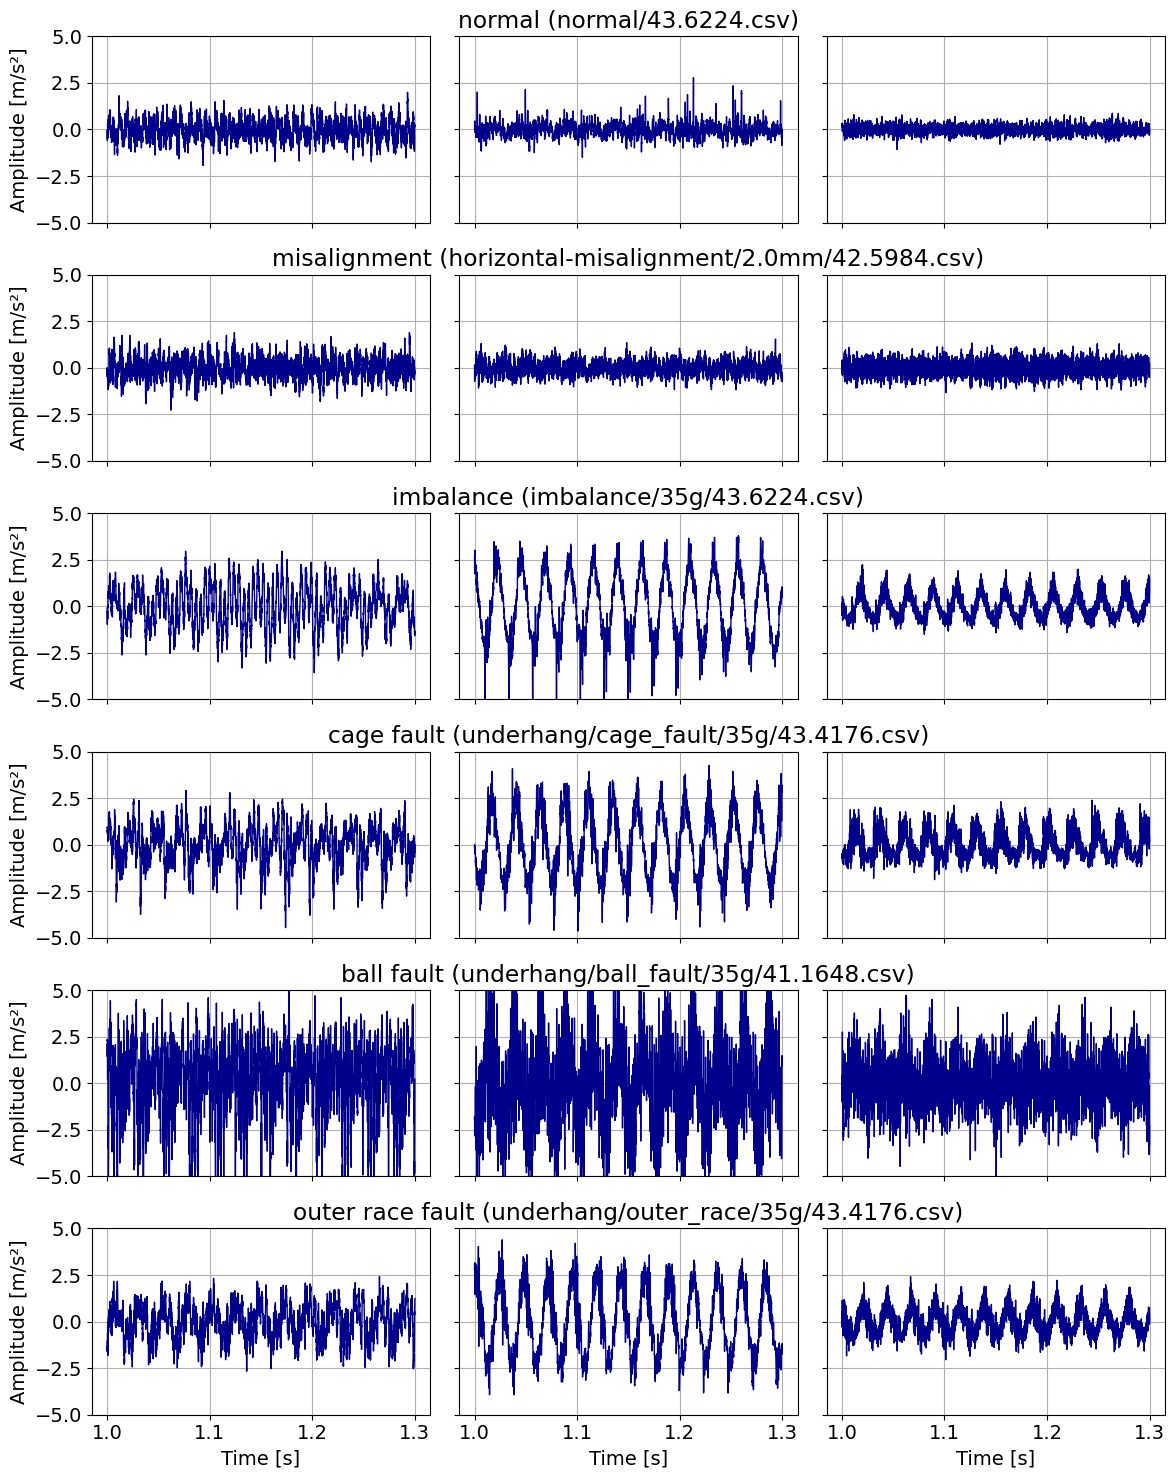
\includegraphics[width=\textwidth]{assets/results/eda/mafaulda-TD-A.png}
        \caption{Time domain for all axis}
        \label{fig:design:fault-temporal-waveform}
    \end{subfigure}
    \hfill
    \begin{subfigure}[b]{0.50\textwidth}
        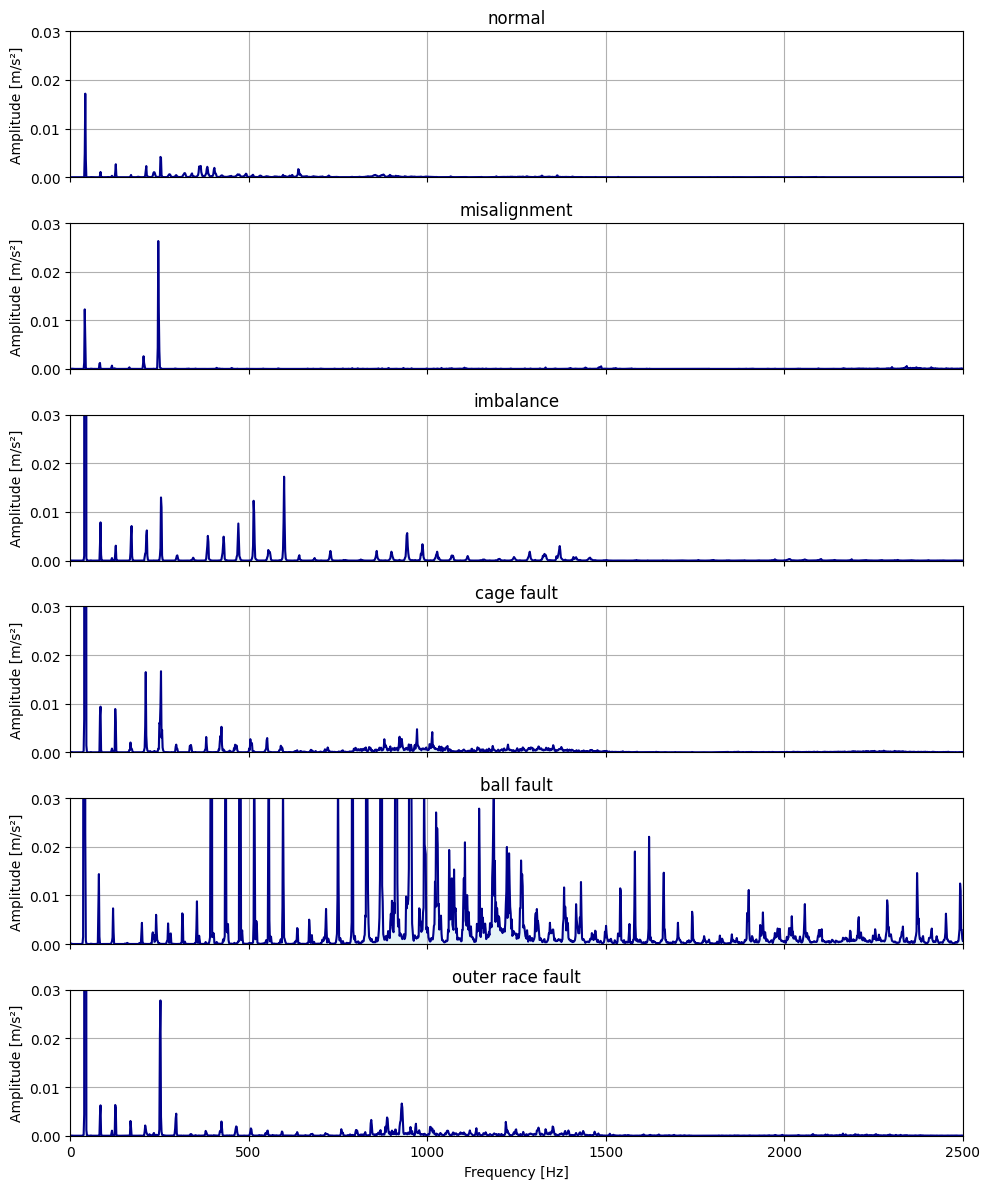
\includegraphics[width=\textwidth]{assets/results/eda/mafaulda-faults.png}
        \caption{Frequency domain in radial direction}
        \label{fig:design:fault-spectral-waveform}
    \end{subfigure}
    \caption{Vibrations from inner bearing (A) for every fault class with the highest fault severity at 2500 rpm}
\end{figure}

Time-domain waveforms of the 300 ms signal slice are shown in the graphs in Figure \ref{fig:design:fault-temporal-waveform}. Subplots for radial, tangential, and axial directions are in columns from left to right. Amplitudes vary with limits from $\pm 3\; \mathrm{m/s}^2$ in baseline and misalignment time series up to $\pm 11\;\mathrm{m/s}^2$ in case of severe bearing faults. 

The frequency spectrum in Figure \ref{fig:design:fault-spectral-waveform} is obtained by FFT and Hann window of 16384 samples. The signal chunk represents an uncertainty box with a duration of approximately 328 ms and a spectral resolution of little over 3 Hz. The graph has been cropped in variables to make the most important peaks visible.

The numeric scale of distinct attributes calculated out of signals for bearing A widely differs ~(Fig.~\ref{fig:design:feature-range}). The magnitude of three spatial dimensions stretches the scale towards larger values or introduces more outliers. Many of the indicators used for fault detection are dimensionless numbers but for others, the information about units of measurement is still attainable. 

\begin{figure}[h]
    \centering
    \begin{subfigure}[b]{0.48\textwidth}
        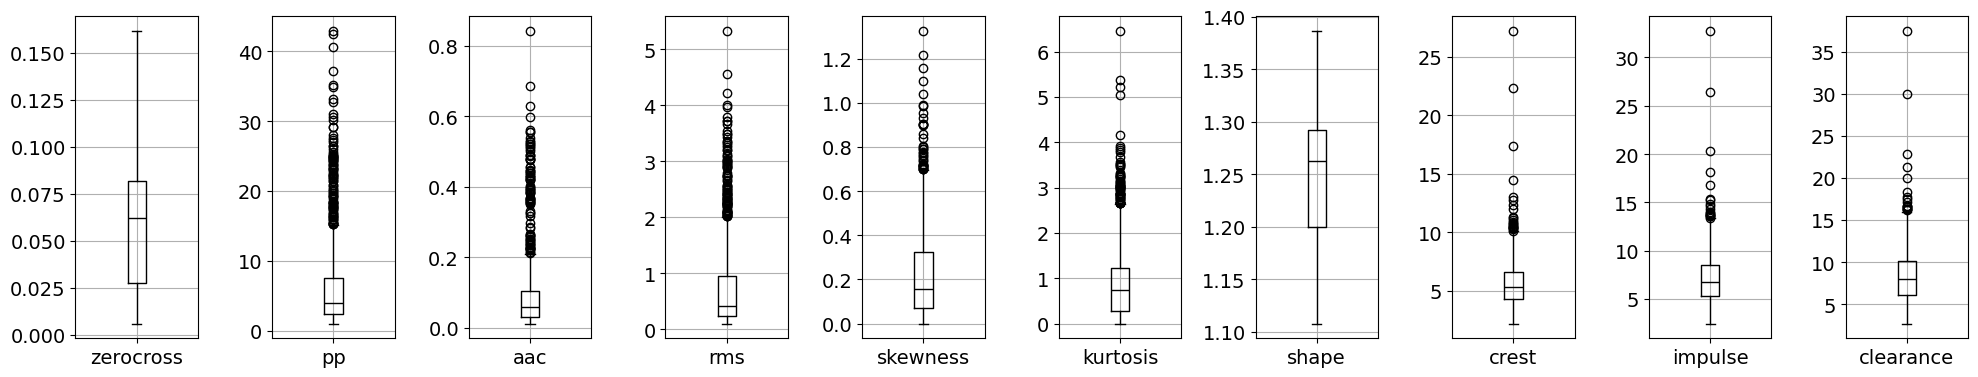
\includegraphics[width=\textwidth]{assets/results/feature-values/features-TD-dim1-A.png}
        \caption{Time-domain features for 1 axis}
    \end{subfigure}
    \hfill
    \begin{subfigure}[b]{0.48\textwidth}
        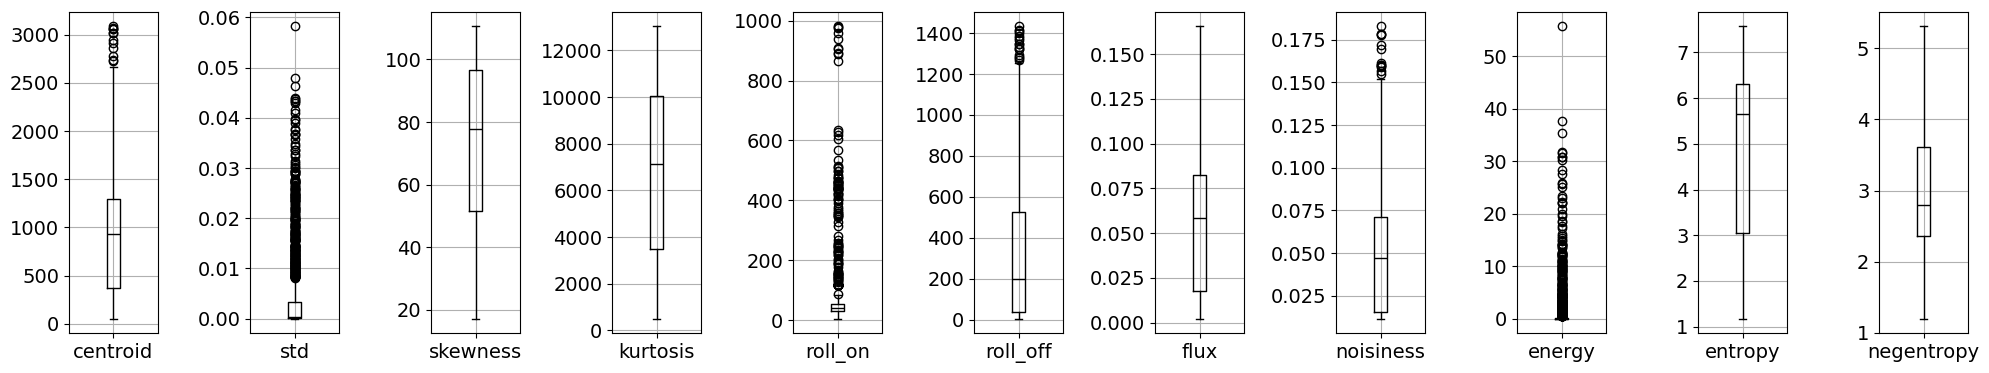
\includegraphics[width=\textwidth]{assets/results/feature-values/features-FD-dim1-A.png}
        \caption{Frequency-domain features for 1 axes}
    \end{subfigure}
    \begin{subfigure}[b]{0.48\textwidth}
        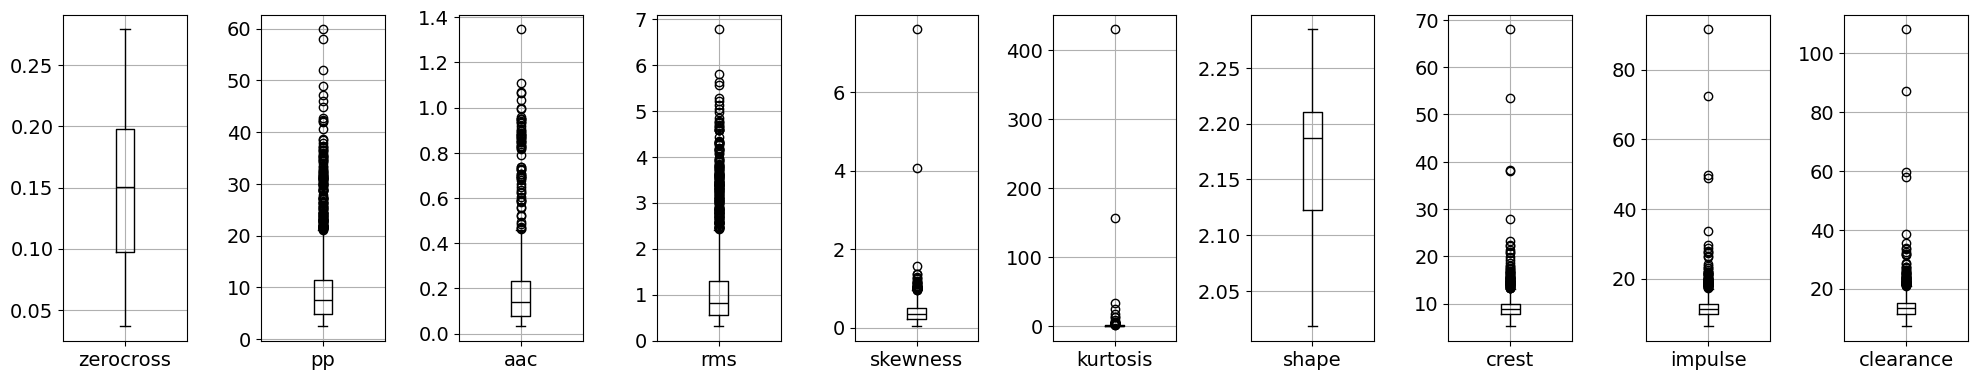
\includegraphics[width=\textwidth]{assets/results/feature-values/features-TD-dim3-A.png}
        \caption{Time-domain features for 3 axes}
    \end{subfigure}
    \hfill
    \begin{subfigure}[b]{0.48\textwidth}
        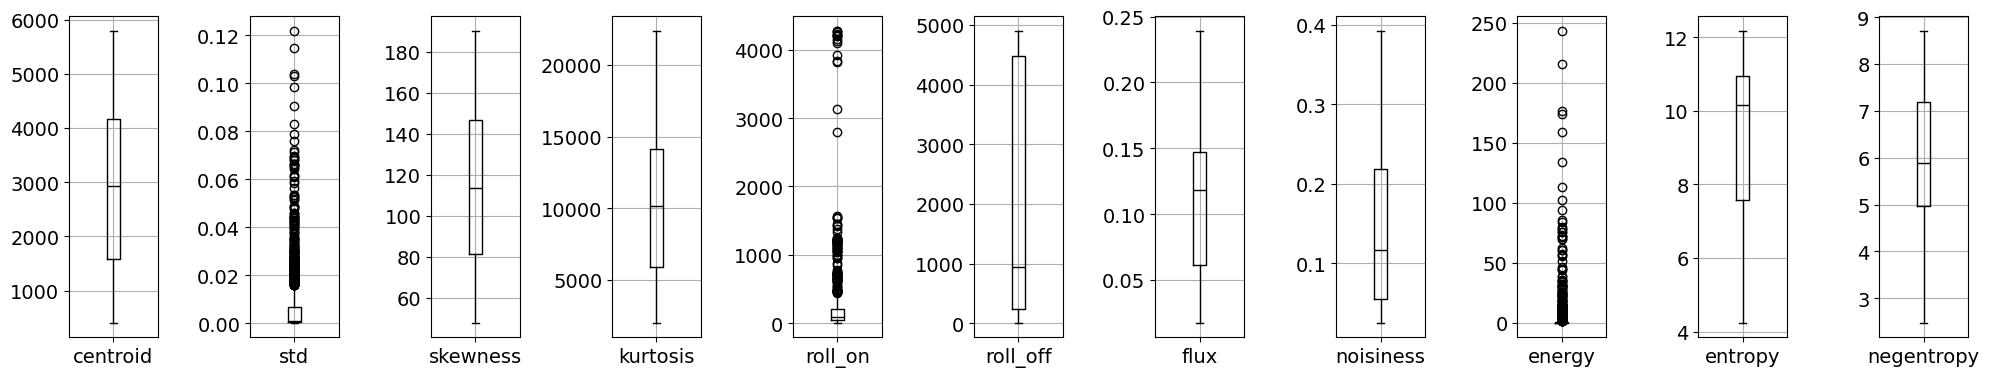
\includegraphics[width=\textwidth]{assets/results/feature-values/features-FD-dim3-A.png}
        \caption{Frequency-domain features for 3 axes}
    \end{subfigure}
    \caption{The value ranges of attributes for bearing A, depending on the number of directions that feature is aggregated out of}
    \label{fig:design:feature-range}
\end{figure}

Inside the interquartile range of three axis features the peak-to-peak is between 4.89 - 11.39 $\mathrm{m/s}^2$, root-mean-square is 0.56 - 1.31 $\mathrm{m/s}^2$, average amplitude change represents 0.08 - 0.23 $\mathrm{m/s}^2$ of amplitude change in 20 $\mu\mathrm{s}$. In the frequency domain, the spectral centroid is in range of 1575 - 4175 Hz, roll-off frequencies arise above 246 and below 4476 Hz, roll-on frequencies are from 50 to 207 Hz, and entropy occurs from 7.57 to 10.94 nats.

Despite the differences in ranges in some instances by several orders of magnitude, there are still dependencies among variables in the complete feature sets. The TD set~(Fig.~\ref{fig:design:corr-td}) appears to have less strongly correlated pairs than the FD set~(Fig.~\ref{fig:design:corr-fd}) in terms of Pearson correlation coefficient. 

\begin{figure}[h]
    \centering
    \begin{subfigure}[b]{0.48\textwidth}
        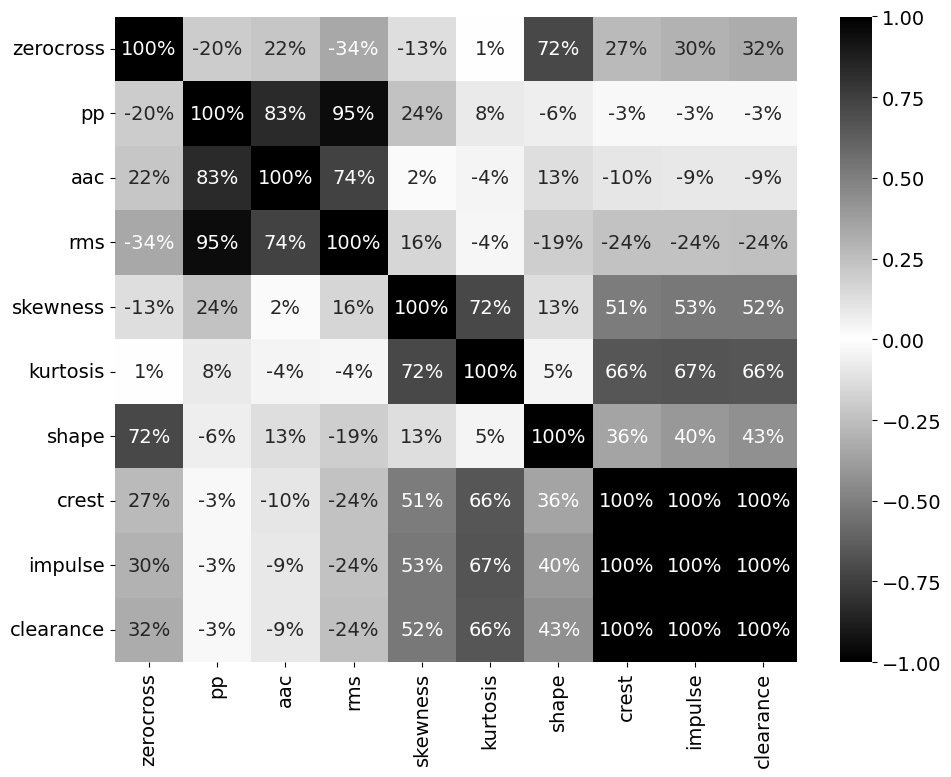
\includegraphics[width=\textwidth]{assets/results/feature-values/corr-A-3-TD.png}
        \caption{Time-domain features}
        \label{fig:design:corr-td}
    \end{subfigure}
    \hfill
    \begin{subfigure}[b]{0.48\textwidth}
        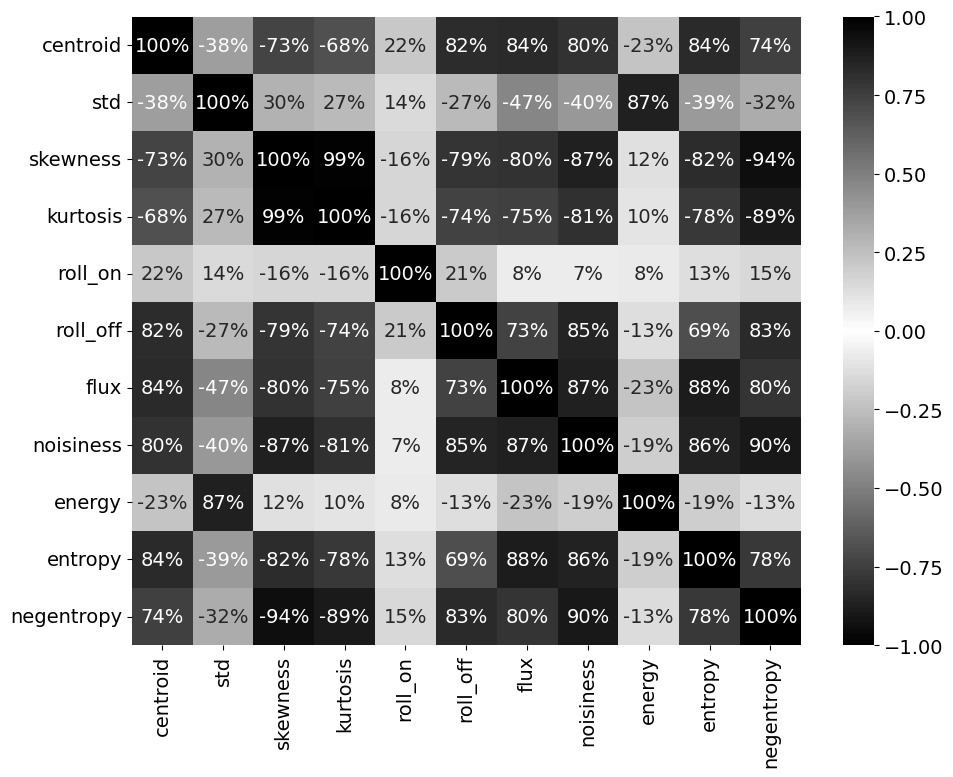
\includegraphics[width=\textwidth]{assets/results/feature-values/corr-A-3-FD.png}
        \caption{Frequency-domain features}
        \label{fig:design:corr-fd}
    \end{subfigure}
    \caption{Pearson correlations of variables from inner bearing (A) in feature sets aggregated out of 3 axes}
\end{figure}

Crest, impulse, and clearance in TD have correlations of 100\%. Other very strongly positively correlated variables are peak-to-peak to root-mean-square at 95\% and average amplitude change at 83\%. Kurtosis is strongly correlated with skewness at 72\% and with crest, impulse, and clearance at 66\%. Shape and zero-crossing rate are also correlated at 72\%. In the FD set the roll-on frequency, energy, and standard deviation are the most uncorrelated to all other variables. However, the energy and std are highly correlated to each other. Skewness and kurtosis of the frequency spectrum have a strong association of 99\%. The rest of the attributes have an absolute value of correlation greater than 68\% in pairs amongst themselves.

\begin{figure}[h]
    \centering
    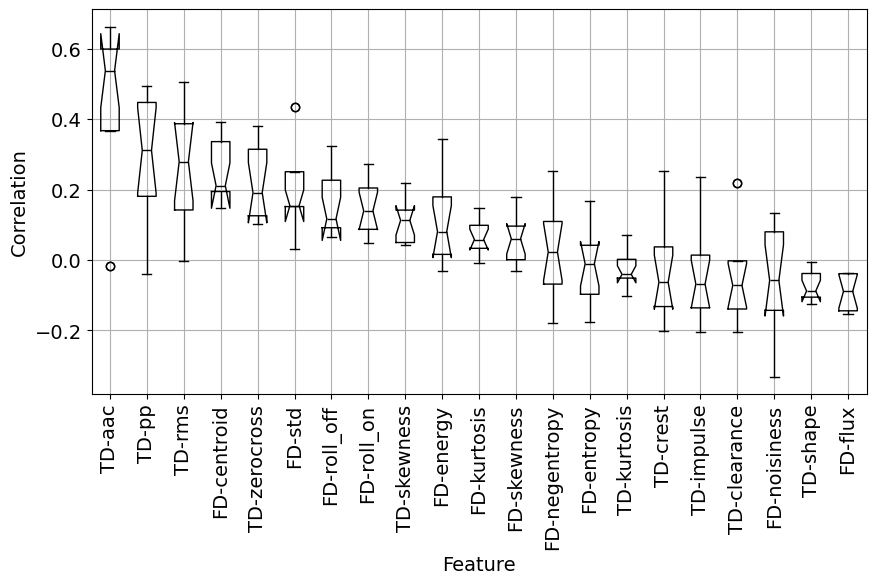
\includegraphics[width=0.8\textwidth]{assets/results/feature-values/corr-to-rpm.png}
    \caption{Correlation of features to rpm over all experiments}
    \label{fig:design:rpm-corr}
\end{figure}

The faults in the MaFaulDa were measured at several rotational speeds. This increases the robustness of the machine-learning model. In practice, if the model is trained only at one speed and then the speed alters, the features tied to rpm could inhibit the prediction accuracy. The distribution of correlations of each predictor to rpm under all experimental conditions is shown in Figure~\ref{fig:design:rpm-corr}. 

The overwhelming majority of predictors are weakly correlated to rotational speed. The moderate correlation appears for average amplitude change with the median of 54\% and peak-to-peak with median of 31\%. These two features are less suited for idenfifying fault types in variable speed situations.

\begin{figure}[h]
    \centering
    \begin{subfigure}[b]{0.48\textwidth}
        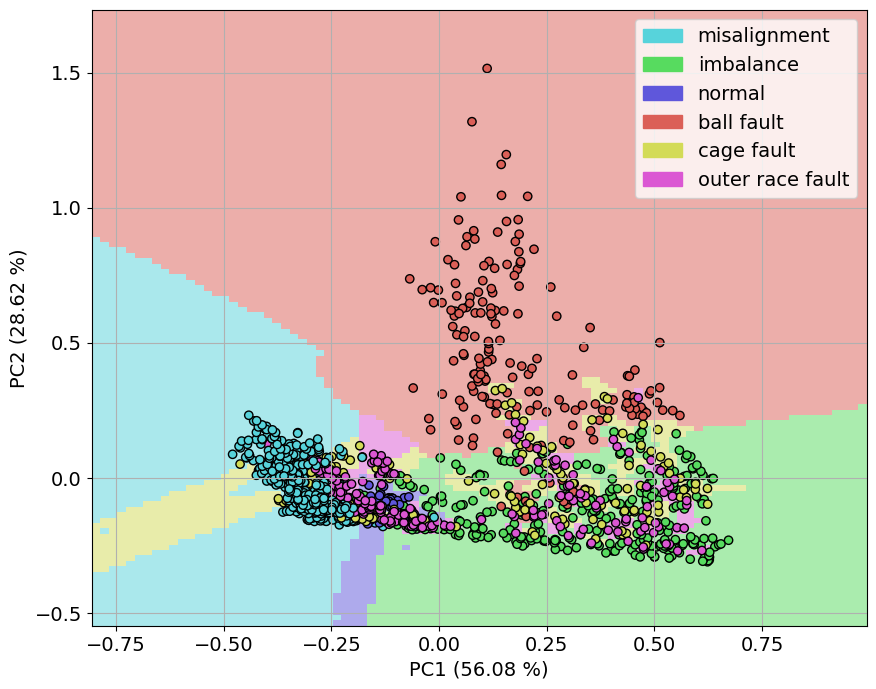
\includegraphics[width=\textwidth]{assets/results/labels/PCA-TD.png}
        \caption{Time-domain features}
    \end{subfigure}
    \hfill
    \begin{subfigure}[b]{0.48\textwidth}
        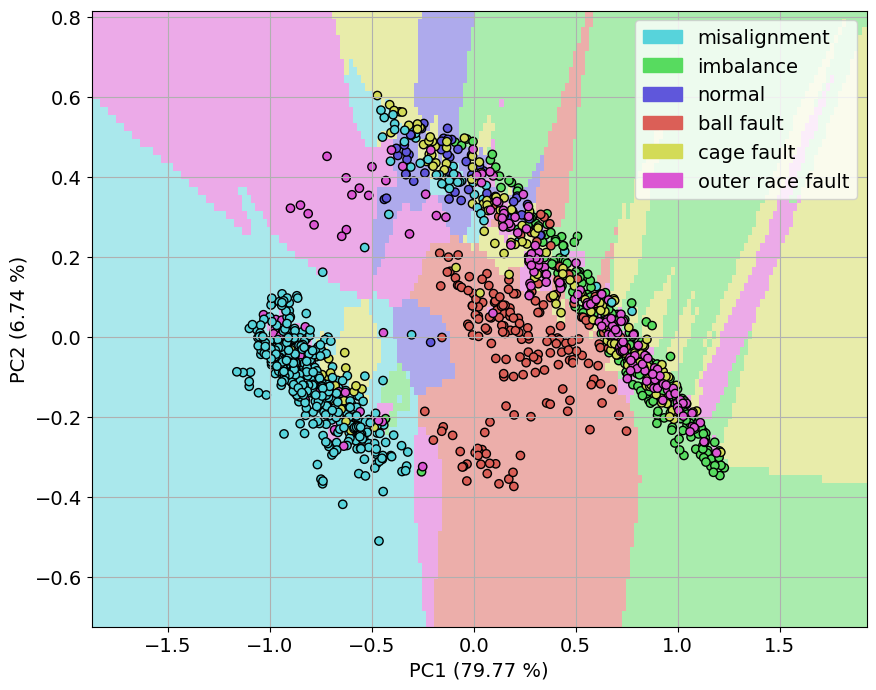
\includegraphics[width=\textwidth]{assets/results/labels/PCA-FD.png}
        \caption{Frequency-domain features}
    \end{subfigure}
    \hfill
    \begin{subfigure}[b]{0.48\textwidth}
        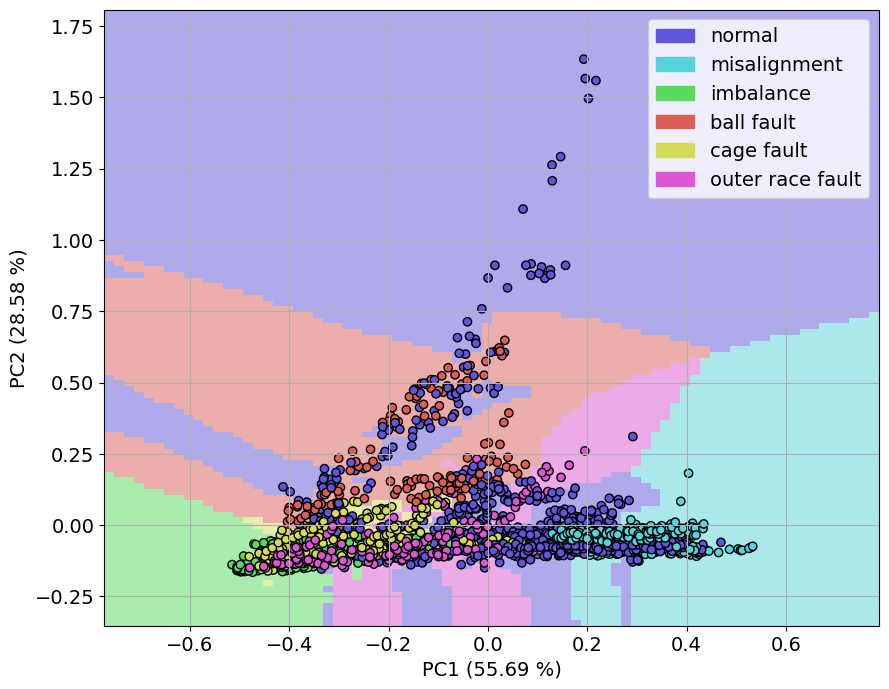
\includegraphics[width=\textwidth]{assets/results/labels/PCA-TD-severity.png}
        \caption{Time-domain features (severity)}
    \end{subfigure}
    \hfill
    \begin{subfigure}[b]{0.48\textwidth}
        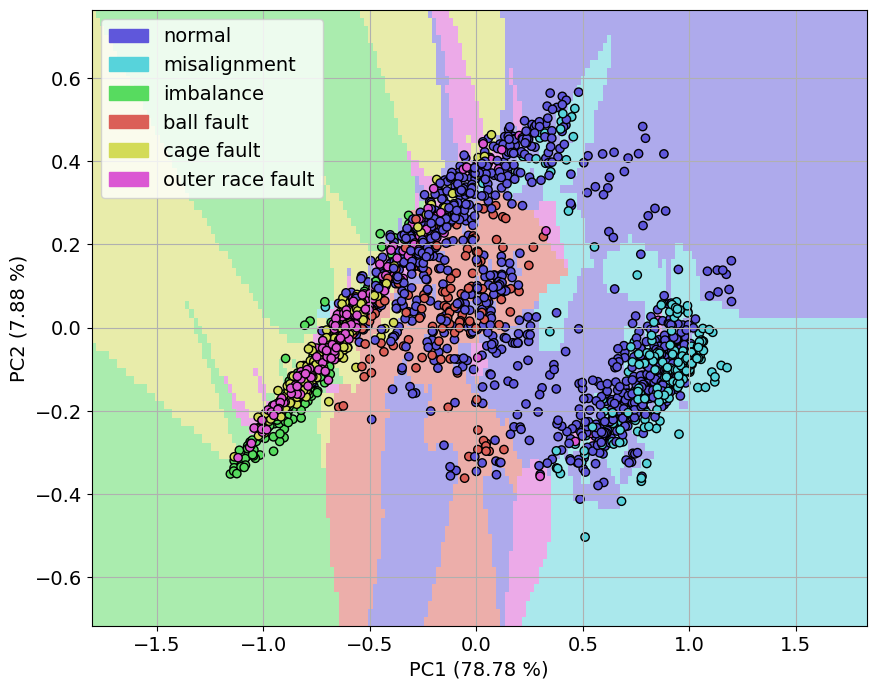
\includegraphics[width=\textwidth]{assets/results/labels/PCA-FD-severity.png}
        \caption{Frequency-domain features (severity)}
    \end{subfigure} 
    \caption{PCA of complete feature set into two principal components (bearing A and 3 axis}
    \label{fig:design:pca-complete-sets}
\end{figure}

The separability of fault groups into clusters is qualitatively analyzed by projecting normalized complete feature sets onto the plain utilizing two principal components. The transformed TD and FD sets are shown in Figure~\ref{fig:design:pca-complete-sets} with original labels and after low severities are assigned ``normal'' class. The decision boundaries that color the feature space around the data points are determined in 0.02x0.02 square areas by k-NN with five neighbours. We observe the inability to separate faults by linear boundaries in given feature spaces and the noncompactness of clusters.

Shaft misalignment and bearing ball fault look quite lumped together, whereas imbalance is mixed with cage fault. The silhouette score quantifies the amount of cluster overlap which indicates a very weak clustering score with values around 0.08. The explained variance with two components is 84.7\% for TD and 86.5\% using original labels.

\begin{figure}[h]
    \centering
    \begin{subfigure}[b]{0.49\textwidth}
        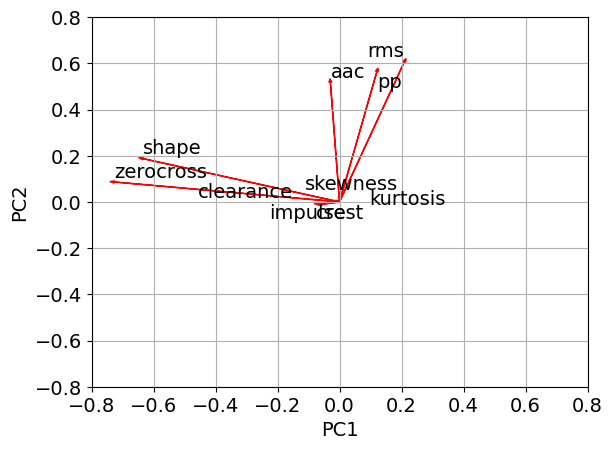
\includegraphics[width=\textwidth]{assets/results/eda/PCA-TD-loading-plot.png}
        \caption{Time-domain features}
    \end{subfigure}
    \hfill
    \begin{subfigure}[b]{0.49\textwidth}
        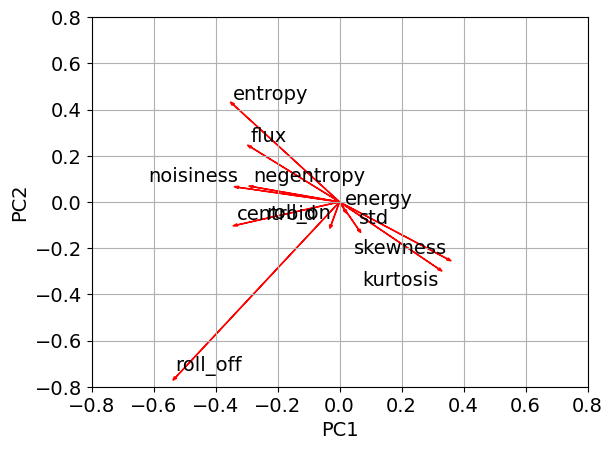
\includegraphics[width=\textwidth]{assets/results/eda/PCA-FD-loading-plot.png}
        \caption{Frequency-domain features}
    \end{subfigure} 
    \caption{PCA loading plots for bearing A}
    \label{fig:design:pca-loading-plot}
\end{figure}

Loading plots of PCA (Fig.~\ref{fig:design:pca-loading-plot}) illustrate correlations of features to two principal components. The first PC in the time domain mainly describes the impulsiveness of the waveform: \emph{shape, impulse, crest, clearance, zero-crossing rate}. The second PC focuses more on the amplitude range: \emph{rms, peak-to-peak, aac}. 

However, the groups are not as clear-cut for frequency-domain features. Overall chaos in frequency spectra can be attributed to PC1: \emph{flux, entropy, negentropy, noisiness}, and the shape of frequency distribution to PC2: \emph{roll-on, roll-off}. PCA efficiently expresses attributes in less dimensional space, but the resulting linear combination is hard to comprehend for explaining decisions. 

\section{Accelerometer data logger}
Data acquisition of vibrations from industrial machinery necessitates the assembly of the standalone data logger. The required hardware modules of the device include a sensor as a triaxial MEMS accelerometer, a fast persistent memory unit, and a microcontroller to control communication with both peripherals. The recording starts with a button press, and the indicator LED provides feedback about the operation in progress. 

More detailed specification according to standards creates demands especially on the accelerometer, in terms of bandwidth for linear response to at least 1 kHz, ideally more. The sampling rate should be greater than 2 kHz for each of the three axes (6 kSps). Out of the options available on the market, we opted for the accelerometers with digital communication bus with more than 12-bit sample resolution, high sensitivity, and low noise density.

\begin{table}[h]
\renewcommand{\arraystretch}{1.2}
\centering
\begin{tabular}{|l|l|l|}
\hline
\textbf{Accelerometer}                   & \textbf{IIS3DWB}   \\ \hline
\textbf{Vendor}                          & STMicroelectronics \\ \hline
\textbf{Bus}                             & SPI  (to 10 MHz)               \\ \hline
\textbf{Axis}                            & 1 or 3             \\ \hline
\textbf{Range}                           & $\pm$ 2 - 16 g (19 - 157 $\mathrm{m/s}^2$)   \\ \hline
\textbf{Bandwidth}                       & 5 - 6.3 kHz           \\ \hline
\textbf{Sensitivity}                     & 0.06 - 0.49 mg/LSB      \\ \hline
\textbf{Noise density} & 75 $\mu \mathrm{g} / \sqrt{\mathrm{Hz}}$ rms                \\ \hline
\textbf{Output data rate}               & 26.8 kHz             \\ \hline
\textbf{Sample resolution}              & 16 bit                 \\ \hline
\textbf{FIFO}                           & 3 kB (512 samples) \\ \hline
\textbf{Microcontroller}                & \textbf{ESP32-PoE-ISO}      \\ \hline
\textbf{CPU SoC}                                 & ESP32-WROOM-32     \\ \hline
\textbf{CPU clock rate}                          & 80 MHz     \\ \hline
\end{tabular}
\caption{Hardware parameters of accelerometer data logger}
\label{tab:design:hw-sensors}
\end{table}

The hardware configuration we arrived at for the data logger powered with a power bank via USB connector is in Table~\ref{tab:design:hw-sensors}. The IIS3DWB accelerometer is a cheap enough MEMS accelerometer that approaches industrial standards for vibration monitoring. The evaluation board for the accelerometer STEVAL-MKI208V1K is connected via a ribbon cable that enables proper attachment to designated places.

\begin{figure}[h]
	\centering
	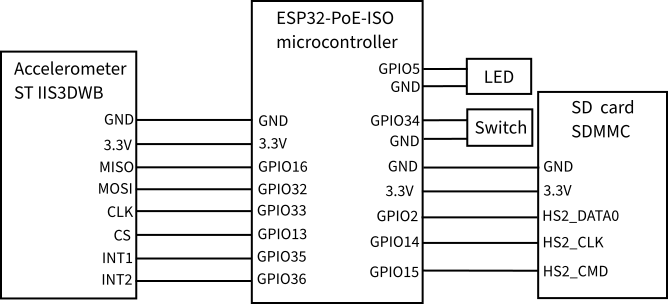
\includegraphics[width=0.9\textwidth]{assets/design/hw-block-schematic.png}
	\caption{Data logger hardware block diagram}
	\label{fig:design:block-diagram-hw}
\end{figure} 

ESP32-PoE-ISO is chosen as a microcontroller development kit because it has an SD card slot connected via an SD/MMC bus. It enables us to store all samples from FIFO. The accelerometer uses an SPI bus with a maximum speed of 10 MHz that can be connected to any physical GPIO pin. The block diagram of the designed hardware device is in Figure~\ref{fig:design:block-diagram-hw}.

\begin{figure}[h]
    \centering
	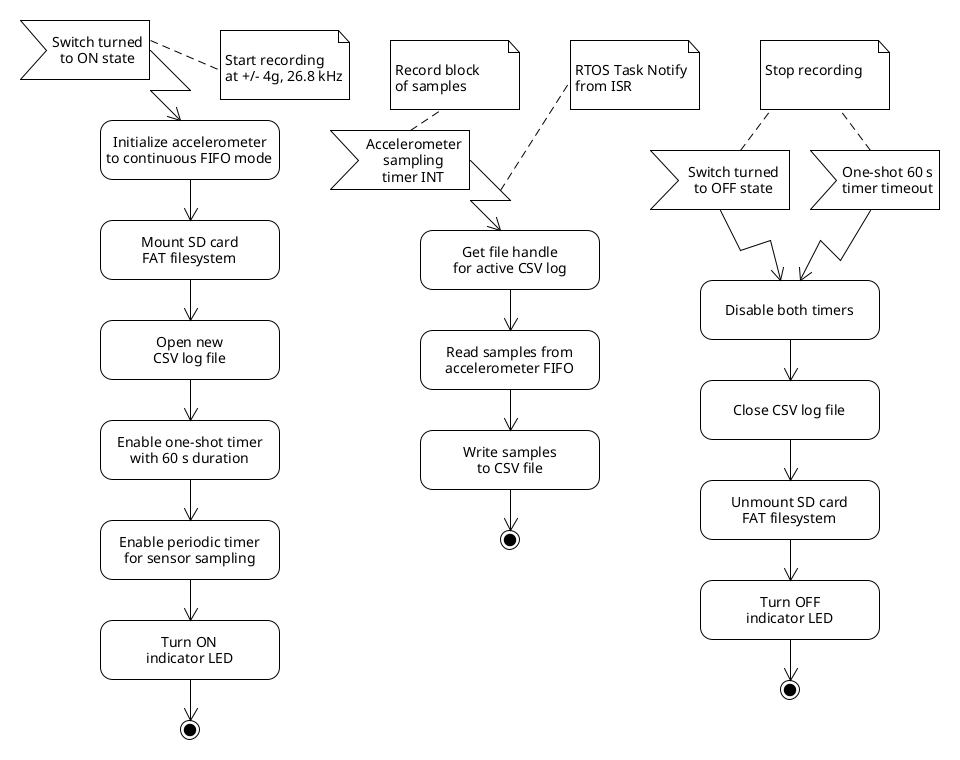
\includegraphics[width=\textwidth]{assets/design/firmware-design.png}
	\caption{Activity diagram of data logger firmware functions}
	\label{fig:design:firmware-activity}
\end{figure}

The firmware's role lies in coordinating hardware adapters and straightforward vibration acquisition for later analysis. The provided functionality is hence minimalistic. Two user-driven actions, one periodic event, and one timer-generated event satisfy these basic requirements. Activity diagrams outline the steps of the firmware actions~(Fig.~\ref{fig:design:firmware-activity}).

\section{Industrial equipment}
Three kinds of rotating machines are at disposal for vibration measurements. Those are a standing fan, scroll compressor, and water pump.

\begin{figure}[h]
    \centering
    \begin{subfigure}[b]{0.3\textwidth}
        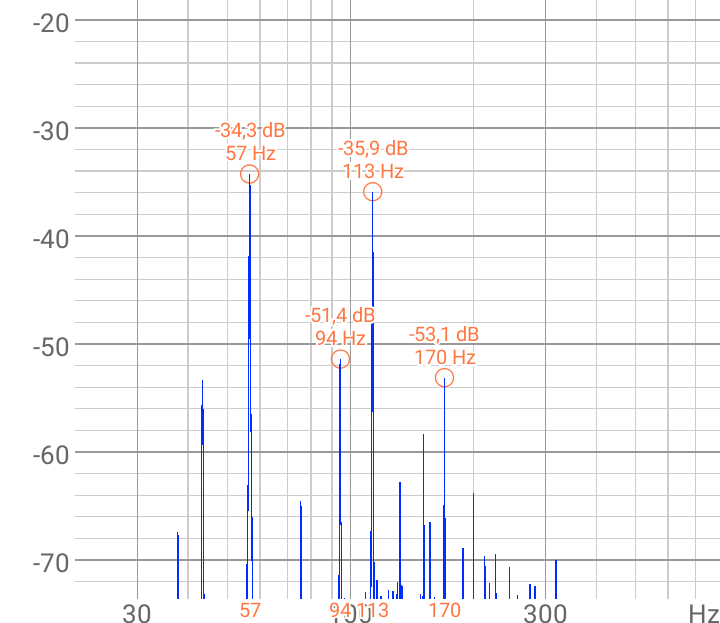
\includegraphics[width=\textwidth]{assets/results/standing-fan/fan-audio-speed-1.png}
        \caption{Fan speed 1}
    \end{subfigure}
    \hfill
    \begin{subfigure}[b]{0.3\textwidth}
        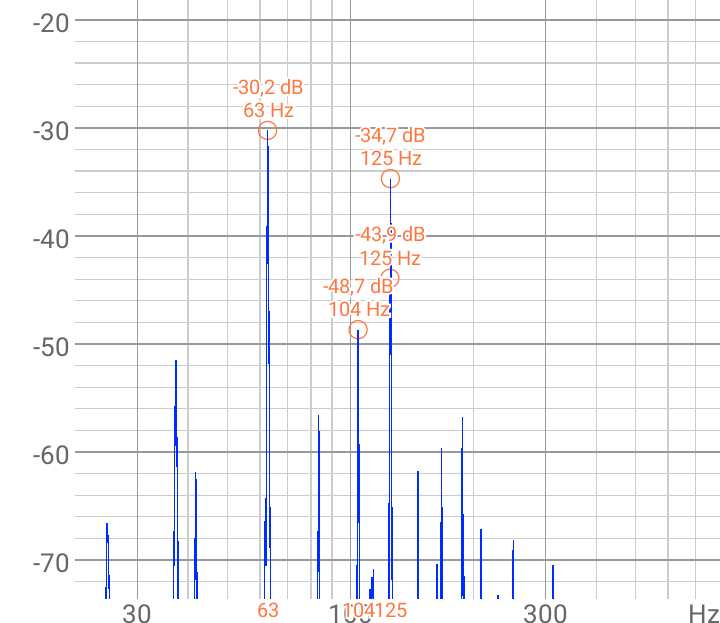
\includegraphics[width=\textwidth]{assets/results/standing-fan/fan-audio-speed-2.png}
        \caption{Fan speed 2}
    \end{subfigure}
    \hfill
    \begin{subfigure}[b]{0.3\textwidth}
        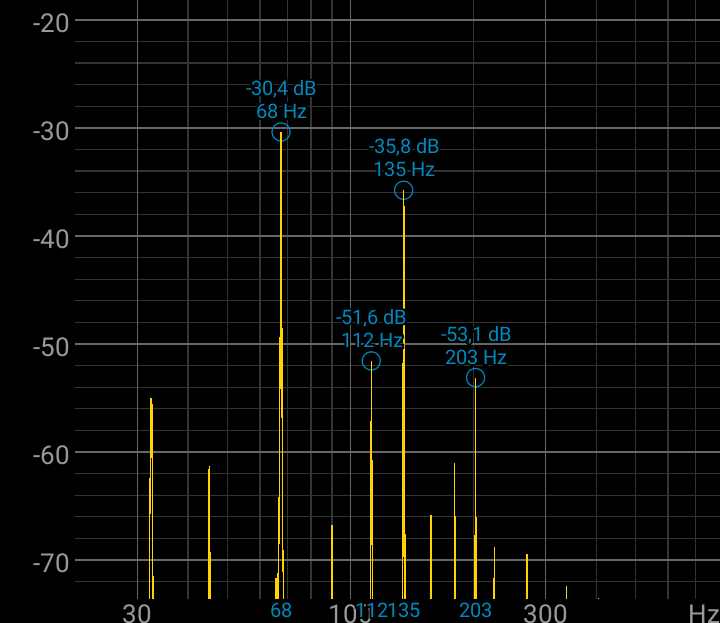
\includegraphics[width=\textwidth]{assets/results/standing-fan/fan-audio-speed-3.png}
        \caption{Fan speed 3}
    \end{subfigure}
    \caption{Frequency spectrum of audio recorded in close proximity to the side of the standing fan}
    \label{fig:design:fan-speed}
\end{figure}

\begin{figure}[h]
    \centering
    \begin{subfigure}[b]{0.49\textwidth}
    		\centering
        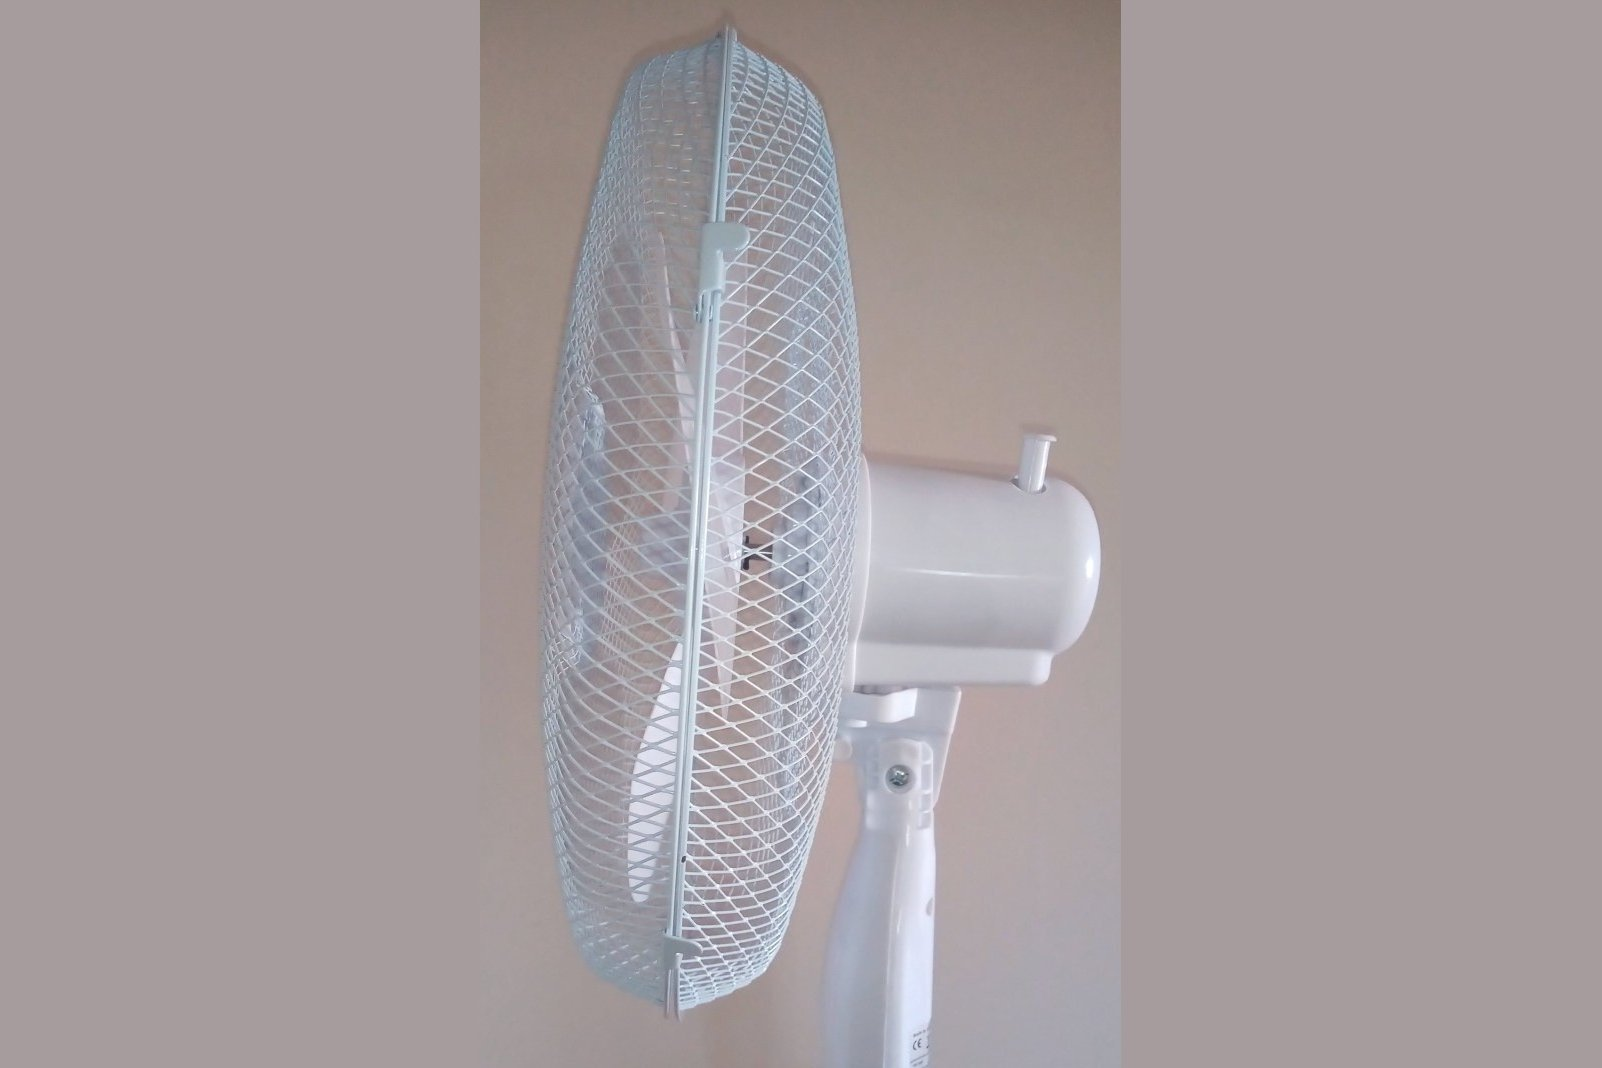
\includegraphics[width=\textwidth]{assets/design/sensor/standing-fan.jpg}
        \caption{\footnotesize Fan}
        \label{fig:machine:fan}
    \end{subfigure}
    \hfill
    \begin{subfigure}[b]{0.49\textwidth}
    		\centering
        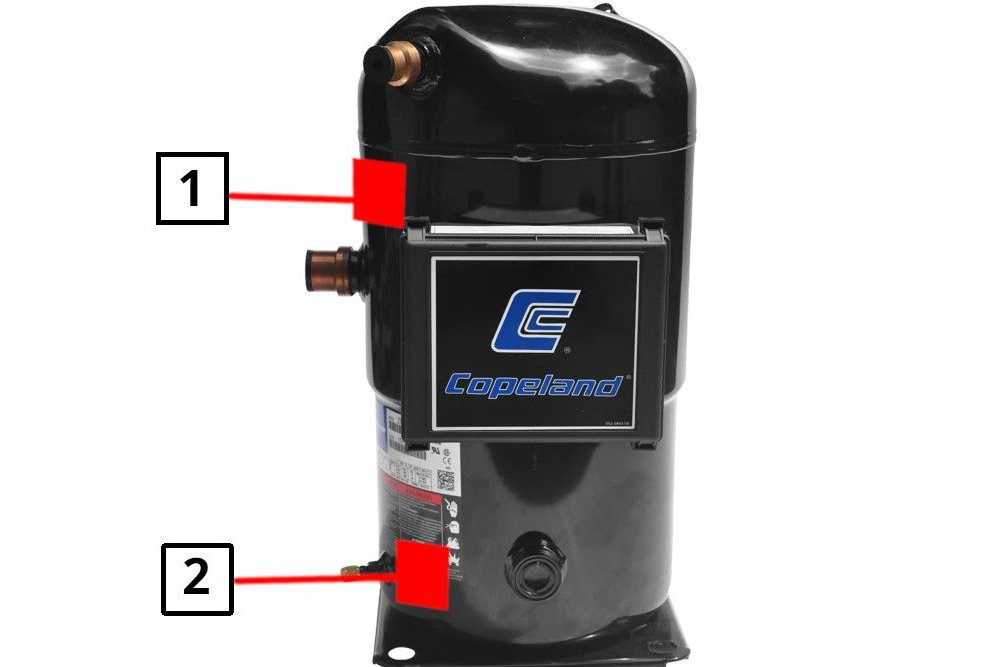
\includegraphics[width=\textwidth]{assets/design/sensor/compressor.jpg}
        \caption{\footnotesize Compressor}
        \label{fig:machine:compressor}
    \end{subfigure}
    \hfill
    \begin{subfigure}[b]{0.49\textwidth}
    		\centering
        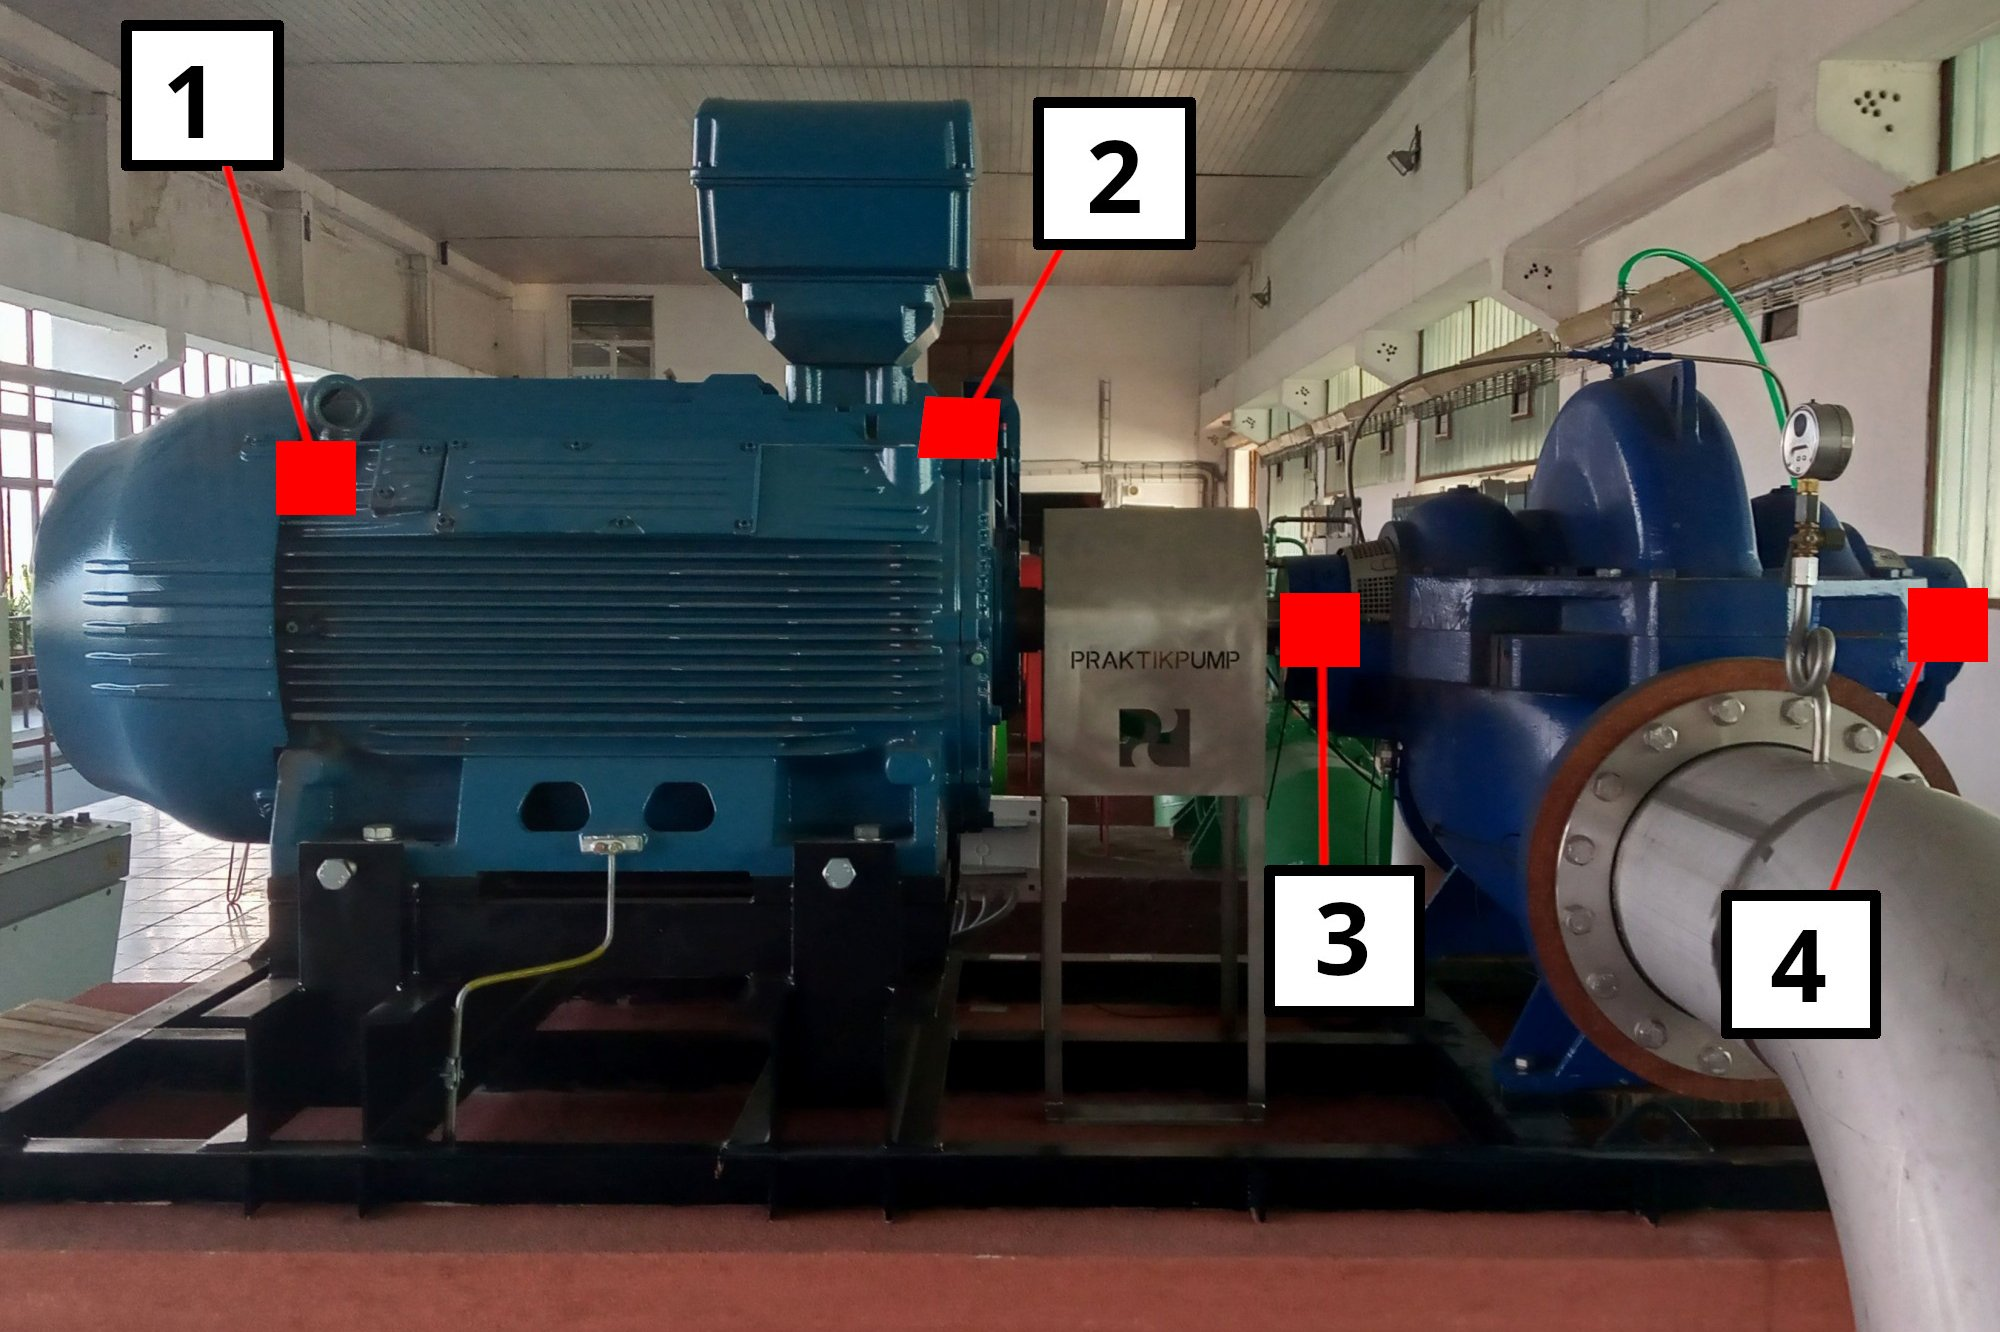
\includegraphics[width=\textwidth]{assets/design/sensor/ksb-pump.jpg}
        \caption{\footnotesize Water pump KSB}
        \label{fig:machine:pump-ksb}
    \end{subfigure}
    \hfill
    \begin{subfigure}[b]{0.49\textwidth}
    		\centering
        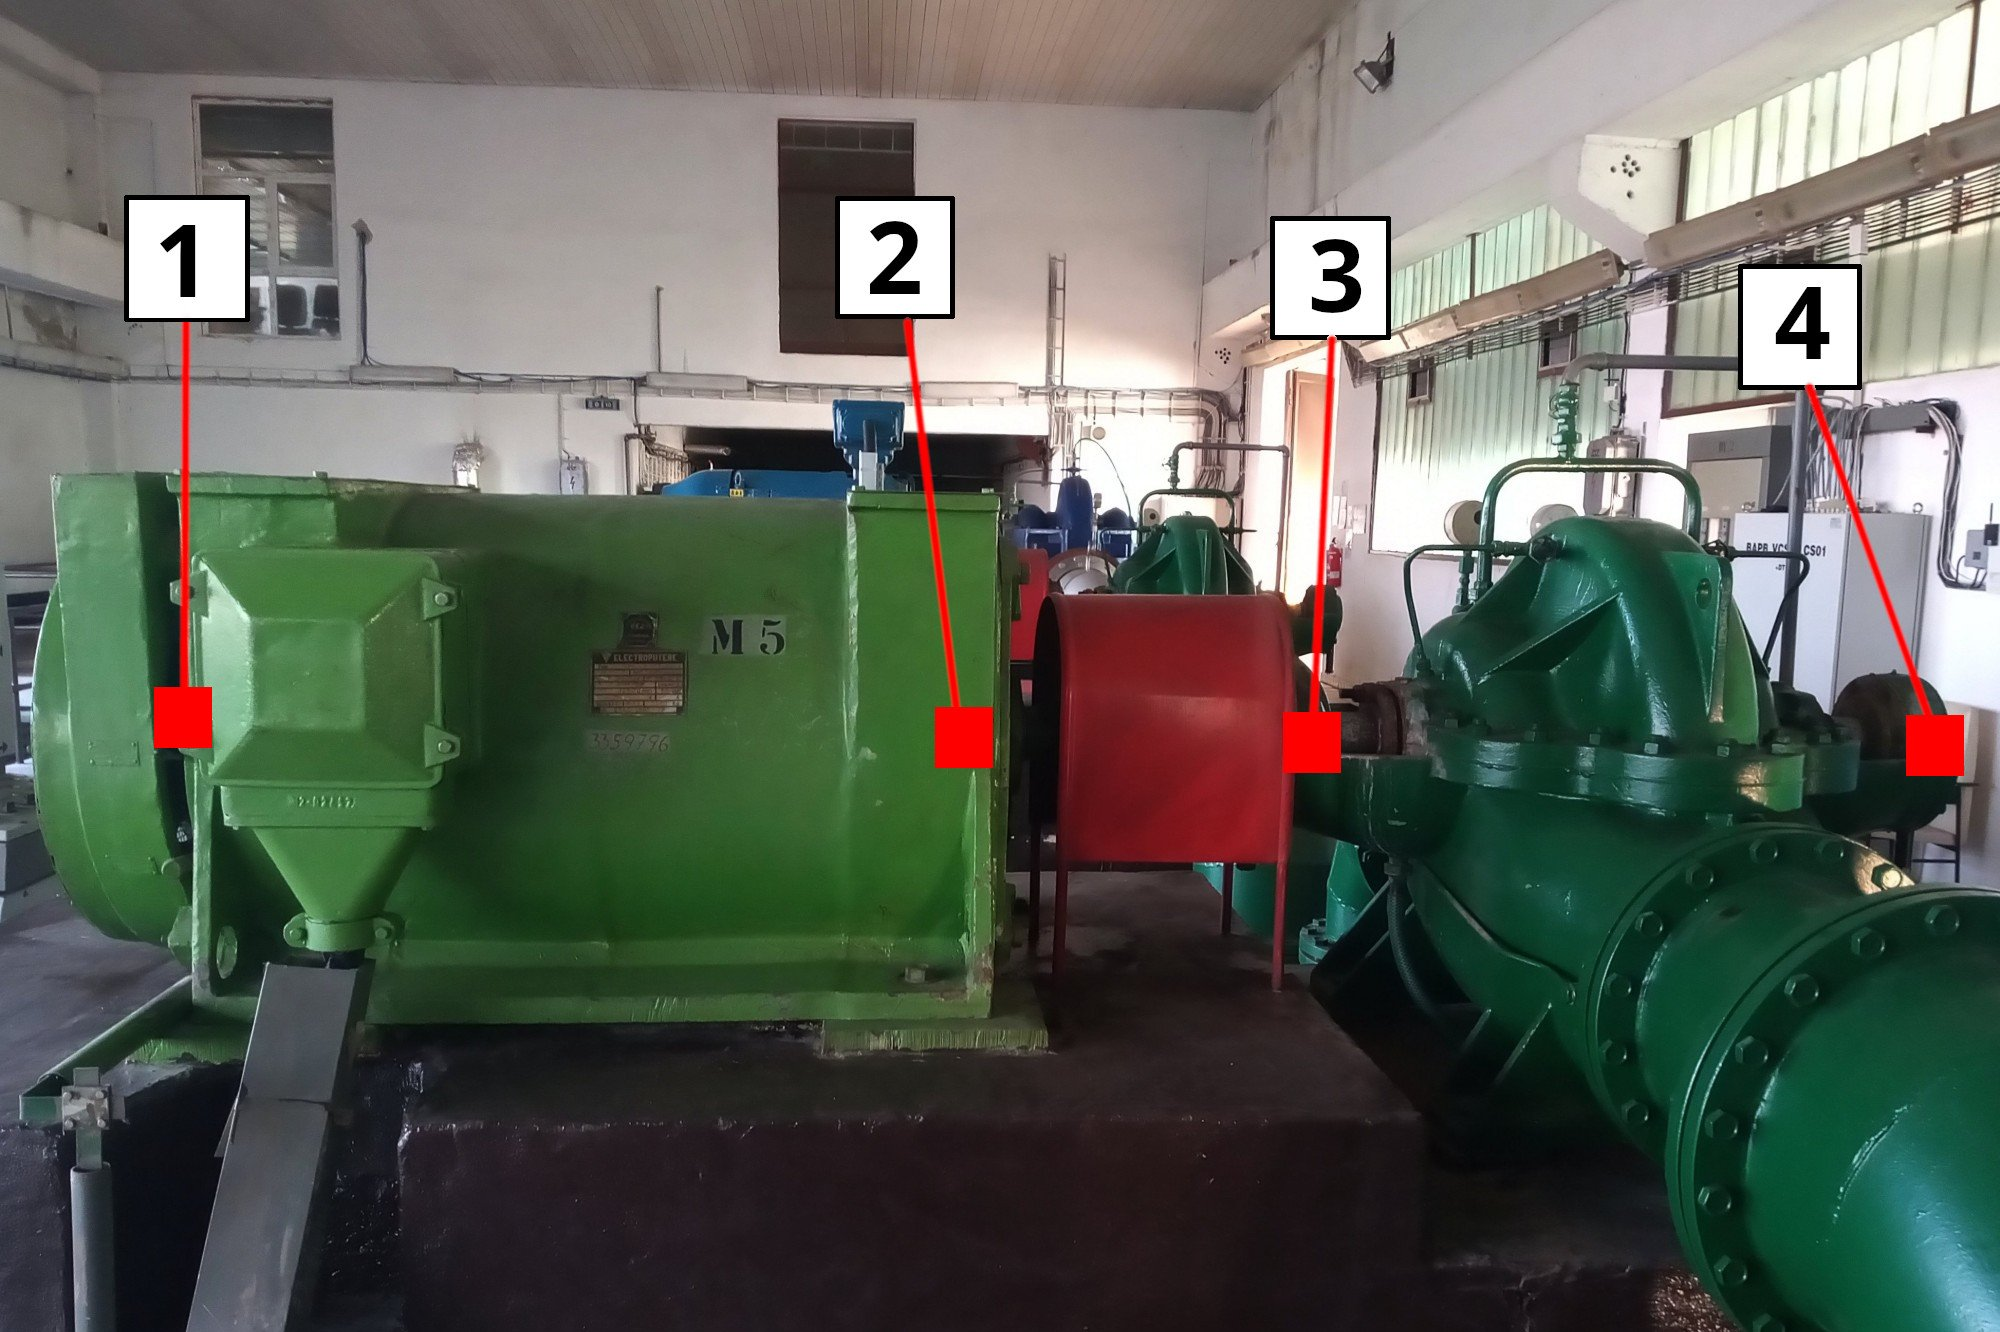
\includegraphics[width=\textwidth]{assets/design/sensor/sigma-pump.jpg}
        \caption{\footnotesize Water pump Sigma}
        \label{fig:machine:pump-sigma}
    \end{subfigure}
    \caption{Machines dedicated for vibration measurements}
    \label{fig:design:machines}
\end{figure}

\textbf{Standing fan} is model \emph{Kalorik~TKG~VT1037} (Fig.~\ref{fig:machine:fan}) and one unit is available to us. It serves as a test bed during the data logger development. The sensor is placed on the plastic casing at the back of the drive motor. The fan has a 45~cm diameter with 3~propellers and a power of 45~W (class~\rom{1}). It has a switch for 3 rotational speeds, which are approximately 19~Hz, 21~Hz, and 22.7~Hz ($\Delta f$ = 0.18 Hz). Speed estimation was done by spectral analysis of audio (Fig.~\ref{fig:design:fan-speed}) in \emph{Spectroid} app and confirmed by 240 fps high-speed camera.

\textbf{Scroll compressor} is model \emph{Copeland~ZR16} (Fig.~\ref{fig:machine:compressor}). Altogether, two units are available in two independent air conditioning units for the data center. The compressor has 9.7~kW of power (class~\rom{1}) and rotates at 2900 rpm (48.3 Hz). Possible measurement locations are located on the sides of the compressor atop the bearings, just above the base and below the scroll. Steel casing is not in direct contact with the bearing which causes significant alteration to the signal.

\textbf{Water pumps} are available as three units in municipal drinking water pumping station. The apparatus consists of a single-stage axially split volute casing pump and an attached electric induction motor. The newer primary pumps with bundled wireless cloud monitoring are two units of \emph{KSB Omega~300-560} (Fig.~\ref{fig:machine:pump-ksb}). The pumps were commissioned in 2018, and they rotate at 1493 rpm (24.9 Hz). The motor \emph{WEG W50} provides 400~kW of power (class~\rom{3}). The bearing designations at numbered places for defect frequency  calculations are 6319-C3 (1), 6324-C3 (2), and 6317-2Z (3 \& 4)

The secondary pump is one unit named \emph{Sigma~300-OVD-600} (Fig.~\ref{fig:machine:pump-sigma}) installed in 1986. It rotates at 1485 rpm (24.75 Hz), and its electric motor has a power of 450~kW (class~\rom{3}). Each pump and motor have two bearings, hence there are four measurement positions.

\section{Data collection methodology}
Vibration measurement for one placement on the machine involves three trials (two for Sigma pump). After each trial, the sensor is detached and attached again to introduce ``noise''. The sensor is mounted to the machine on a flat surface with adhesive of thin double-sided carpet tape.

Placements are numbered for simplicity (Fig.~\ref{fig:design:machines}) but the precise description follows the notation of MIMOSA convention from ISO~13373-1. The sensor is mounted on compressor's placem: \emph{SFTA001AT000TN} (1), \emph{SFTA002AT000TN} (2), on WEG motor's positions: \emph{MTRA001AT000TN} (1), \emph{MTRA002AT045TN} (2), and on KSB pump positions: \emph{PMPA003AT000TN} (3), \emph{PMPA004AT000TN} (4).

\begin{table}[h]
\renewcommand{\arraystretch}{1.2}
\begin{adjustbox}{width=\columnwidth,center}
\begin{tabular}{|ll|cc|ccc|ccc|}
\hline
\multicolumn{2}{|l|}{\textbf{Machine}}                                     & \multicolumn{2}{l|}{\textbf{Scroll compressor}} & \multicolumn{3}{l|}{\textbf{Water pump}}                                          & \multicolumn{3}{l|}{\textbf{Pump's motor}}                                        \\ \hline
\multicolumn{2}{|l|}{\textbf{Facility code}}                            & \multicolumn{1}{c|}{K3}           & K5          & \multicolumn{1}{c|}{KSB-1}       & \multicolumn{1}{c|}{KSB-7}       & Sigma-5     & \multicolumn{1}{c|}{KSB-1}       & \multicolumn{1}{c|}{KSB-7}       & Sigma-5     \\ \hline
\multicolumn{2}{|l|}{\textbf{Label}}                                       & \multicolumn{1}{c|}{C1}           & C2          & \multicolumn{1}{c|}{P1}          & \multicolumn{1}{c|}{P2}          & P3          & \multicolumn{1}{c|}{M1}          & \multicolumn{1}{c|}{M2}          & M3          \\ \hline
\multicolumn{1}{|l|}{\multirow{5}{*}{\textbf{Date}}} & \textbf{20/02/2024} & \multicolumn{1}{c|}{$\bigtimes$}  & $\bigtimes$ & \multicolumn{1}{c|}{}            & \multicolumn{1}{c|}{}            &             & \multicolumn{1}{c|}{}            & \multicolumn{1}{c|}{}            &             \\ \cline{2-10} 
\multicolumn{1}{|l|}{}                               & \textbf{27/02/2024} & \multicolumn{1}{c|}{}             &             & \multicolumn{1}{c|}{$\bigtimes$} & \multicolumn{1}{c|}{$\bigtimes$} &             & \multicolumn{1}{c|}{$\bigtimes$} & \multicolumn{1}{c|}{$\bigtimes$} &             \\ \cline{2-10} 
\multicolumn{1}{|l|}{}                               & \textbf{05/03/2024} & \multicolumn{1}{c|}{$\bigtimes$}  & $\bigtimes$ & \multicolumn{1}{c|}{}            & \multicolumn{1}{c|}{}            &             & \multicolumn{1}{c|}{}            & \multicolumn{1}{c|}{}            &             \\ \cline{2-10} 
\multicolumn{1}{|l|}{}                               & \textbf{19/03/2024} & \multicolumn{1}{c|}{$\bigtimes$}  & $\bigtimes$ & \multicolumn{1}{c|}{}            & \multicolumn{1}{c|}{}            &             & \multicolumn{1}{c|}{}            & \multicolumn{1}{c|}{}            &             \\ \cline{2-10} 
\multicolumn{1}{|l|}{}                               & \textbf{26/03/2024} & \multicolumn{1}{c|}{}             &             & \multicolumn{1}{c|}{$\bigtimes$} & \multicolumn{1}{c|}{$\bigtimes$} & $\bigtimes$ & \multicolumn{1}{c|}{$\bigtimes$} & \multicolumn{1}{c|}{$\bigtimes$} & $\bigtimes$ \\ \hline
\end{tabular}
\end{adjustbox}
\caption{Data collection schedule}
\label{fig:design:data-schedule}
\end{table}

The triaxial recording has a duration 60~s (at $f_s$ = 26.8~kHz) and a 16-bit resolution. One file has 24.6~MiB as a binary stream and 48~MiB in TSV format. 
Measurements were executed and organized into folders according to schedule in Table~\ref{fig:design:data-schedule}. It should be noted that because of operational regulations, the second KSB pump was measured the day after the first. The estimated total space requirements for all 92 uncompressed raw recordings is 2.21~GiB and approximately 4.31~GiB as TSV files (Tab-separated values). The dataset shall be called \emph{Pump dataset}.

\begin{figure}[h]
    \centering
    \begin{subfigure}[b]{0.49\textwidth}
    		\centering
        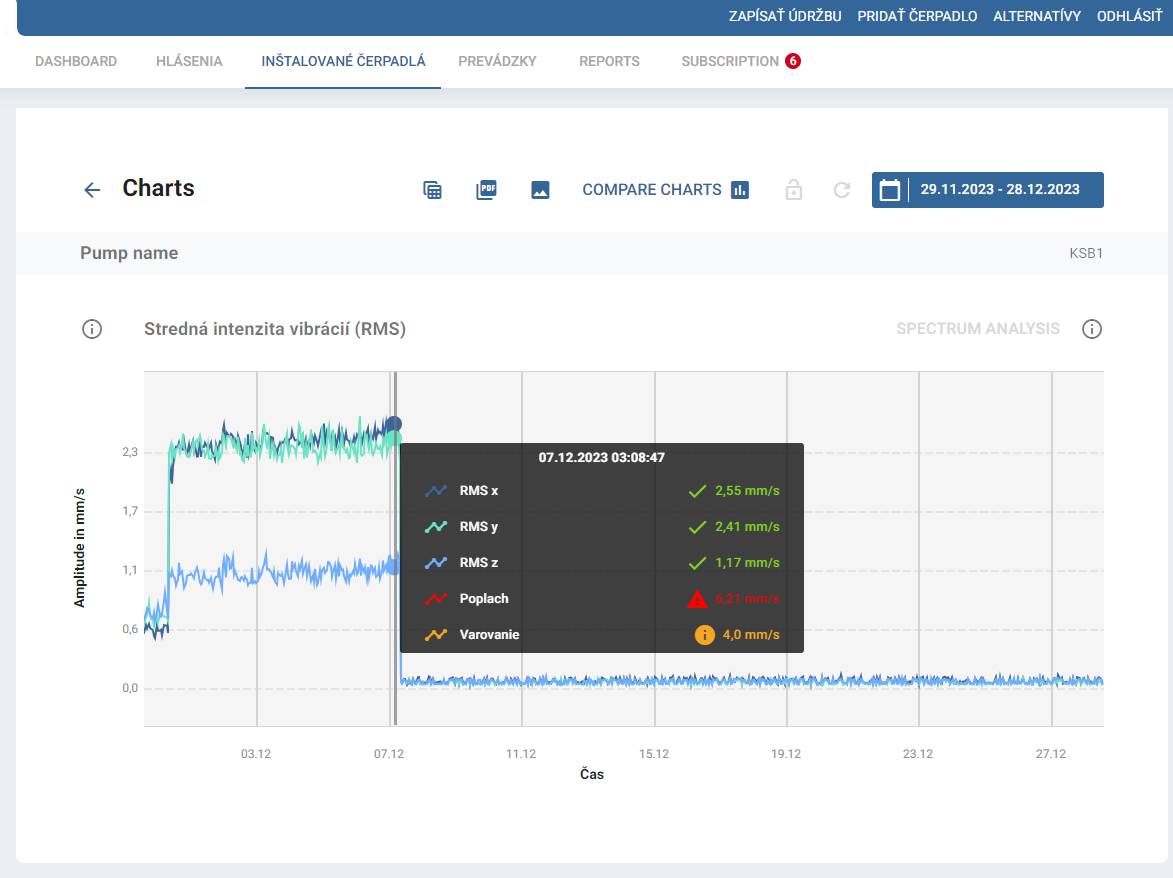
\includegraphics[width=\textwidth]{assets/design/ksb-guard-rms.png}
        \caption{Vibration rms velocity dashboard}
    \end{subfigure}
    \hfill
    \begin{subfigure}[b]{0.49\textwidth}
    		\centering
        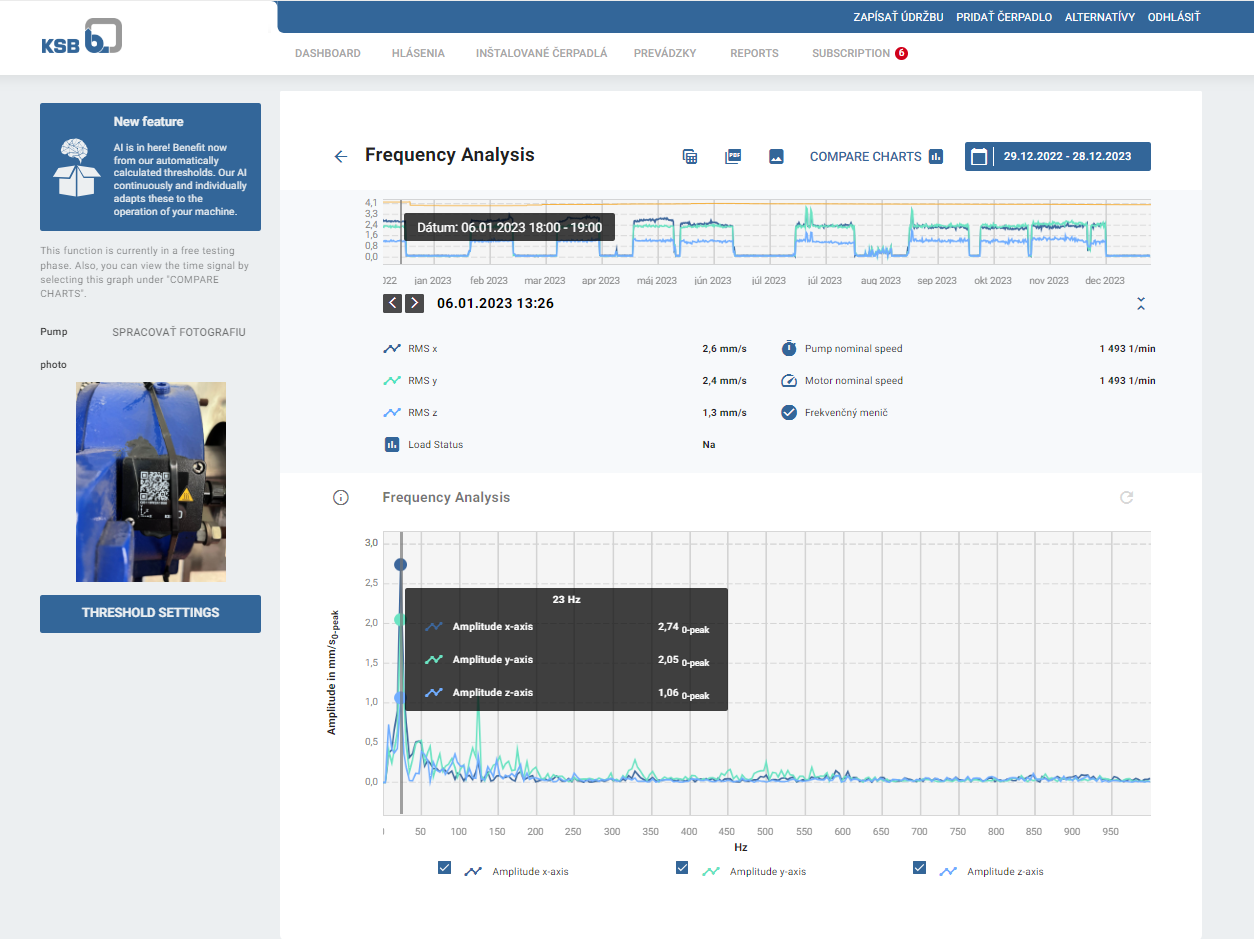
\includegraphics[width=\textwidth]{assets/design/ksb-guard-spectrum.png}
        \caption{Vibration frequency analysis dashboard}
    \end{subfigure}
    \hfill
    \begin{subfigure}[b]{0.49\textwidth}
    		\centering
        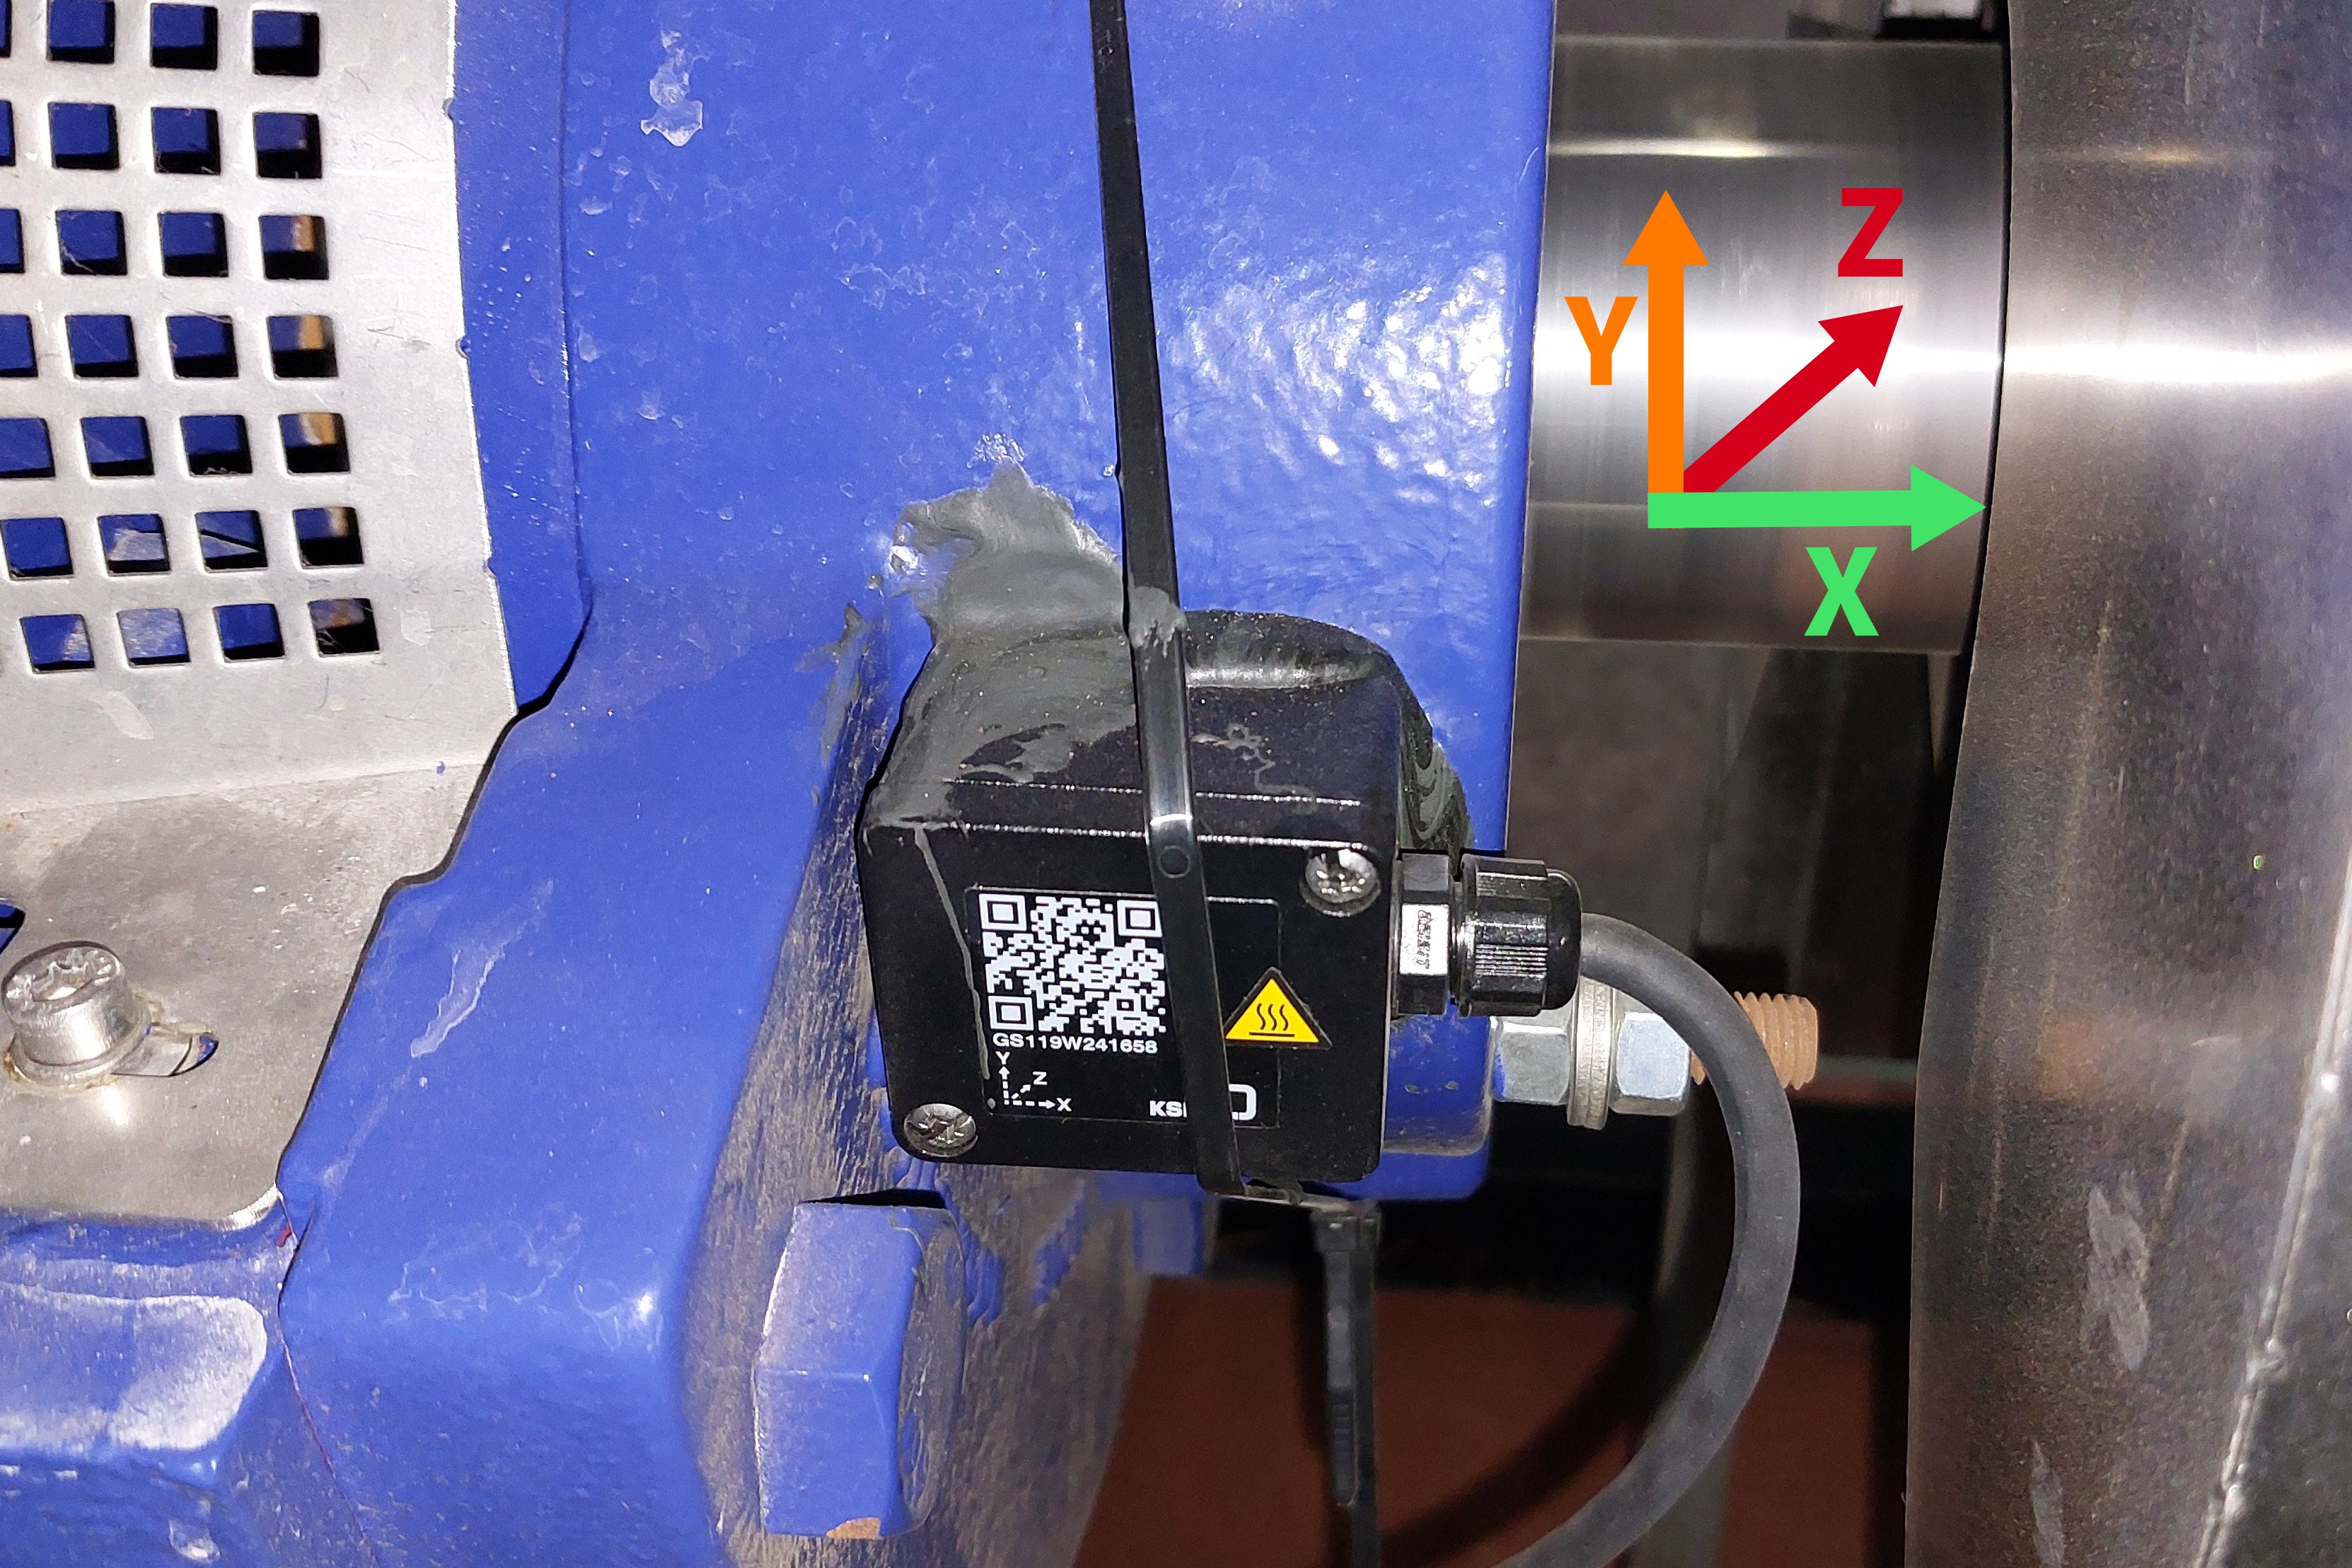
\includegraphics[width=\textwidth]{assets/design/sensor/ksb-cloud.jpg}
        \caption{KSB Guard Sensor Unit}
        \label{fig:design:ksb-device}
    \end{subfigure}
     \caption{KSB Guard cloud monitoring for pumps}
     \label{fig:design:ksb-guard}
\end{figure}

Logs from \textbf{KSB Guard} cloud monitoring tool contain vibration rms velocities and frequency spectra for two monitored KSB water pumps (Figure~\ref{fig:design:ksb-guard}). We were able to export the historical log of vibration velocity for last year at hourly intervals and sample frequency spectra. The sensor unit (Fig.~\ref{fig:design:ksb-device}) is permanently attached to KSB pumps on bearing in position no. 3.

\section{Data volume savings}
The apparent advantage of feature discovery is reducing the amount of data downstream. Data compression must occur on edge devices to enable the utilization of wireless low-power wide area networks (LPWAN). The protocol stack may differ, so goodput in this section is compared without node configuration metadata and keepalive messages. 

The machinery monitoring system relies on determining a few parameters:
\begin{itemize}
\itemsep0pt
\item \textbf{Number of source channels} ($S$) - comprises the number of monitored machines, measurement locations for sensors, and active sensor axes.
\item \textbf{Sampling frequency} ($f_s$) - is set based on the linear response of the accelerometer, the types of faults intended for detection, and how soon they should be noticed after they arise. The higher required sensitivity means a higher sampling rate derived according to the Nyquist theorem. At a minimum, it should be 15 kHz to 20 kHz.
\item \textbf{Interval between successive measurements} ($T$) - specifies the minimal response time to sudden failure. The more critical the machine is, the shorter the interval should be. The bigger the machine parts, the slower the defect evolves.
\item \textbf{Duration of valid recording} ($D$) - is the captured snapshot of machine unaltered behavior associated with a timestamp. Duration should cover at least twelve windows for spectral estimation.
\item \textbf{Number of extracted features} ($F$) - are ideally key trend indicators pointing to symptoms of common malfunctions. We aim for a total of six features.
\end{itemize}

Equation \ref{equ:compression-ratio-features} expresses the lossy compression ratio ($\mathcal{C}$) formula if trend indicators are stored instead of full recording. The number of raw channels ($S_{\mathrm{in}}$) can differ from those extracted in features ($S_{\mathrm{out}}$). Parameter $D = 0.5$ when we use frequency bins with 1 Hz resolution.

\myequations{Lossy compression ratio with features}
\begin{ceqn}\begin{align} \label{equ:compression-ratio-features}
\mathcal{C} = \frac{D \cdot f_s \cdot S_{\mathrm{in}}}{F \cdot S_{\mathrm{out}}}
\end{align}\end{ceqn}

\textbf{Compression ratio} for MaFaulDa dataset compared to all 21 extracted features in 3 dimensions is 2381:1. If 6 features are kept, the compression is 25000:1, which is a saving of the original data by 99.996\%.

As an example to approximate required network goodput and storage in practice, we consider continuous vibration \textbf{monitoring for municipal water pumping station}. The station has three pumps and three electric motors. 

A pump and motor pair have four bearings together for drive end and non-drive end positions. Each position has a sensor mounted in three directions that makes a total of \emph{36 source channels}. The sampling frequency at each position is set to \emph{20 kHz}. The recordings have \emph{duration of five seconds} and are triggered regularly every 1 hour (\emph{8760 times per year}).

In a year, the system gathers 31.54 Gs (gigasamples) which is 58.74 GiB with a 16-bit ADC resolution. Reasonably precise spectral estimation with 10 thousand bins needs 3.15 Gs per year. On the other hand, 6 features out of each channel keep only 1.89 Ms per year for a lossy compression ratio of 16667:1. Low data volumes potentially enable feature selection and models to be offloaded directly to edge devices. The entire history of the machine's health could be stored in a small flash memory module.
